\documentclass{lug}

\title{Computer Graphics}
\author{Sam Sartor}
\institute{Mines Linux Users Group}

\usepackage{etoolbox}
\usepackage{array}
\usepackage{amsmath}
\usepackage{adjustbox}
\usepackage{calc}
\usepackage{lmodern}

\makeatletter
\patchcmd{\beamer@sectionintoc}{\vskip1.5em}{\vskip0.5em}{}{}
\makeatother

\newcommand{\pmidg}[1]{\parbox{\widthof{#1}}{#1}}
\newcommand{\splitslide}[4]{
    \noindent
    \begin{minipage}{#1 \textwidth - #2 }
        #3
    \end{minipage}%
    \hspace{ \dimexpr #2 * 2 \relax }%
    \begin{minipage}{\textwidth - #1 \textwidth - #2 }
        #4
    \end{minipage}
}

\begin{document}

\section{Introduction}

\begin{frame}{Uses}
    \splitslide{0.65}{.7em}{
        Computer graphics is everywhere!
        \begin{itemize}
            \item Your terminal
            \item Web browsers
            \item Video games
            \item CAD software
            \item Movies, TV Shows
            \item Virtual reality
            \item Your bootloader
            \item QT, GTK+, wxWidgets
            \item Vim, Emacs, Notepad
            \item Embedded devices
        \end{itemize}
    }{
        \pmidg{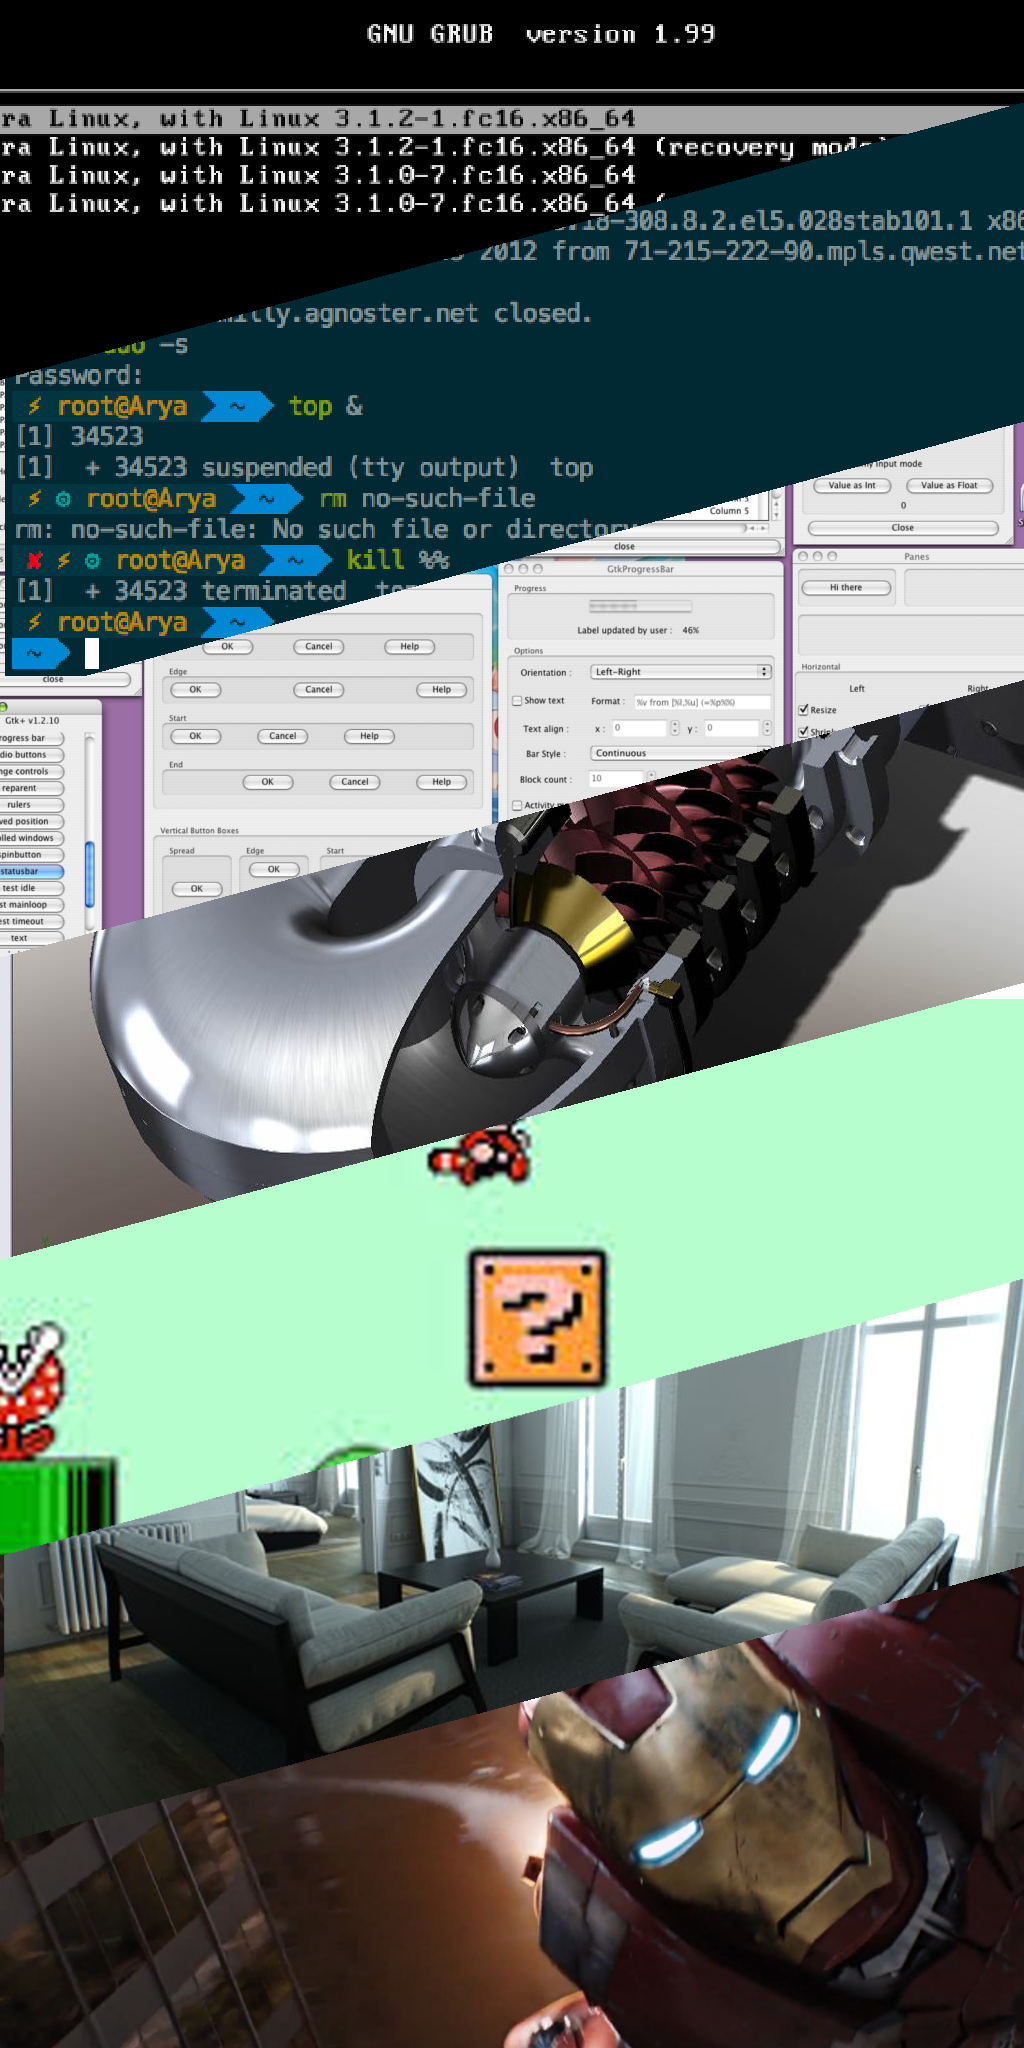
\includegraphics[width=\textwidth]{graphics/uses}}
    }
\end{frame}

\begin{frame}{Definition}
\begin{center}
    \pmidg{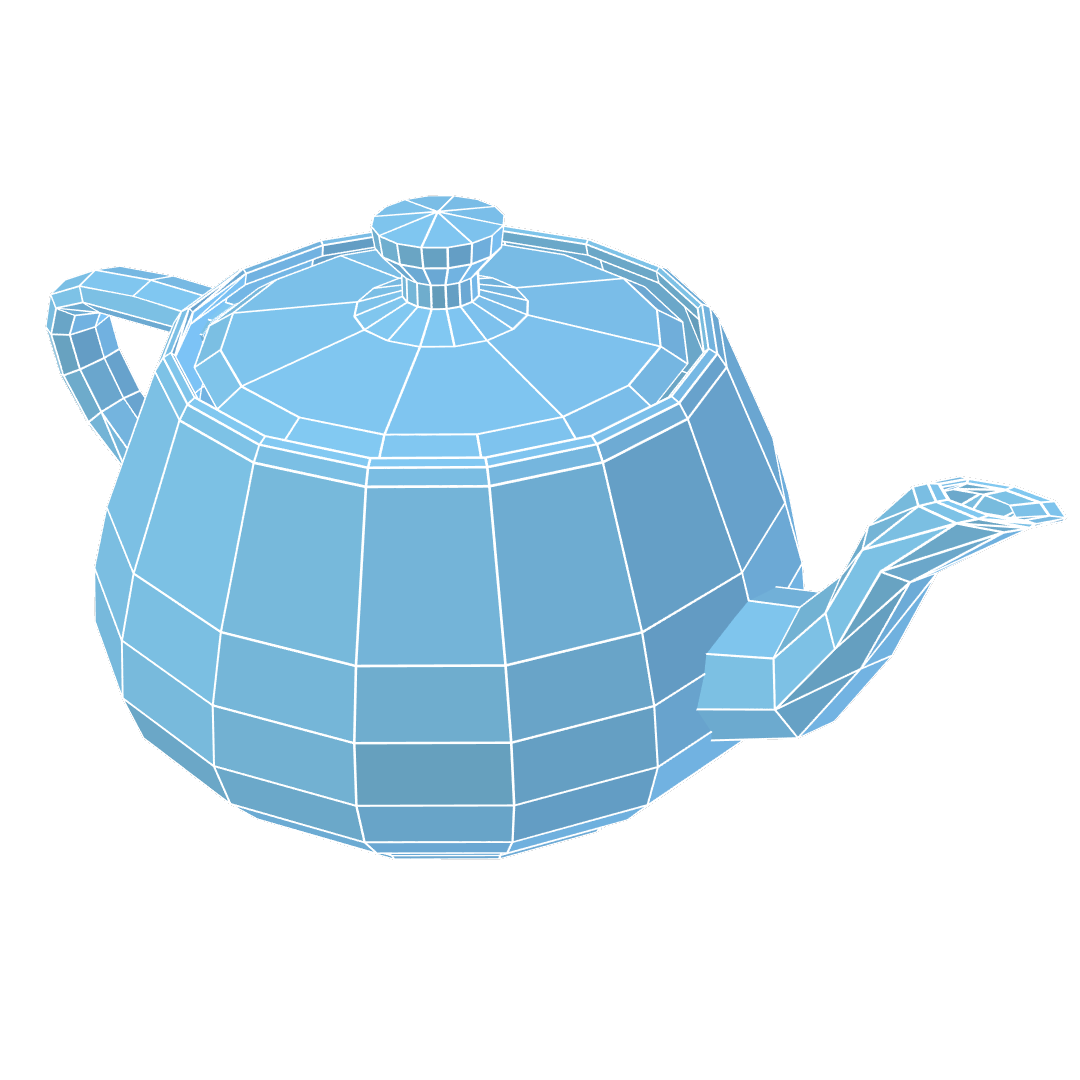
\includegraphics[width=4cm]{graphics/teapot_mesh}} \scalebox{2}{$\rightarrow$} \pmidg{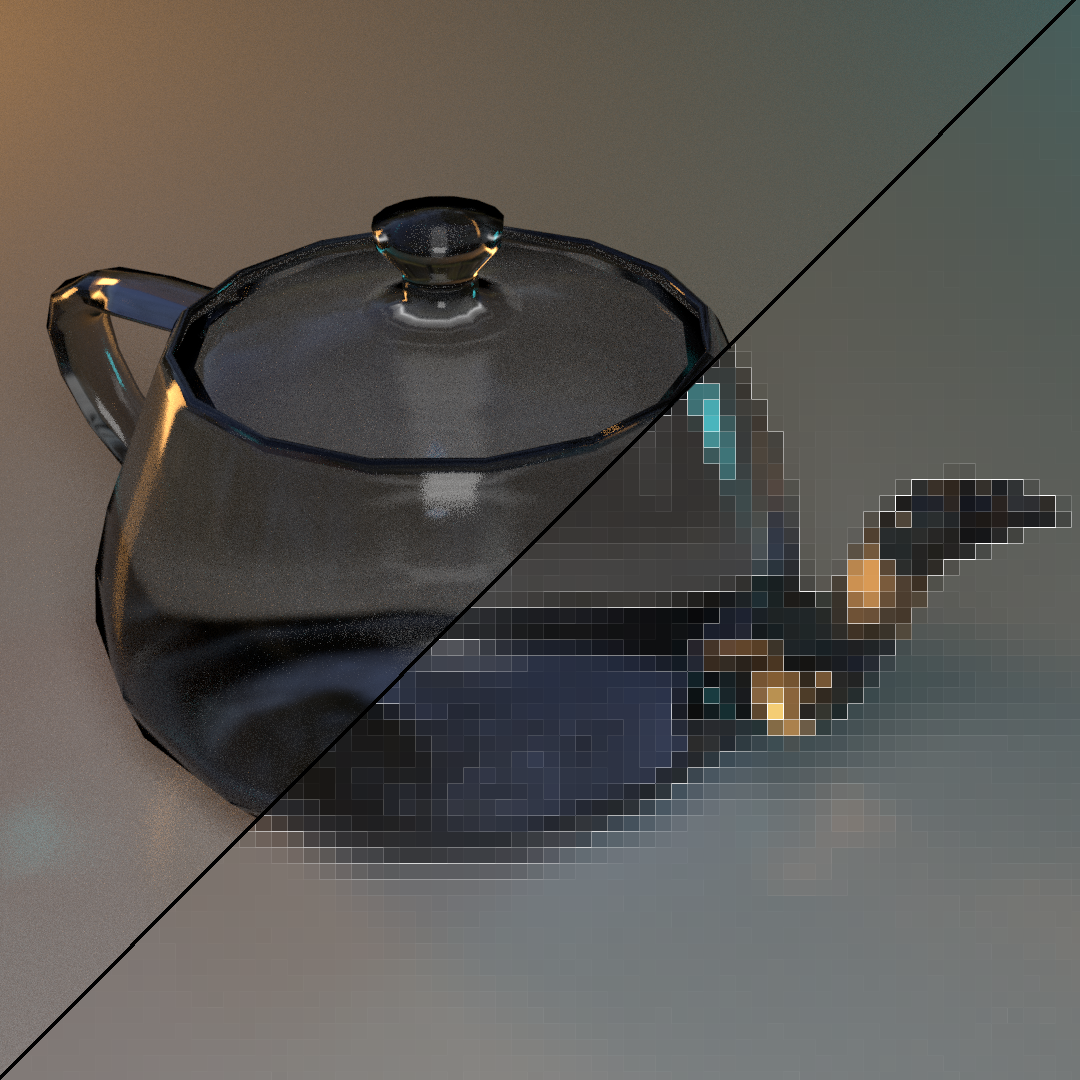
\includegraphics[width=4cm]{graphics/teapot_rt_pix}} \\
    
    \bigskip

    Computer graphics is the science of turning \textit{shapes} into \textit{pixels}. \footnote{Kindof, it can get more interesting than that}
\end{center}
\end{frame}

\section{Behind the Scenes}

\begin{frame}{Realtime}
    \splitslide{0.7}{.7em}{
        \small

        Realtime graphics use OpenGL or Direct3D to rasterize and shade
        triangular geometry on a graphics card/chip. Performance is very
        important due to the high framerate that is required for smooth
        gameplay/interactivity/animation. Lighting and materials focus on
        being "good enough" rather than on being truly accurate.

    }{
        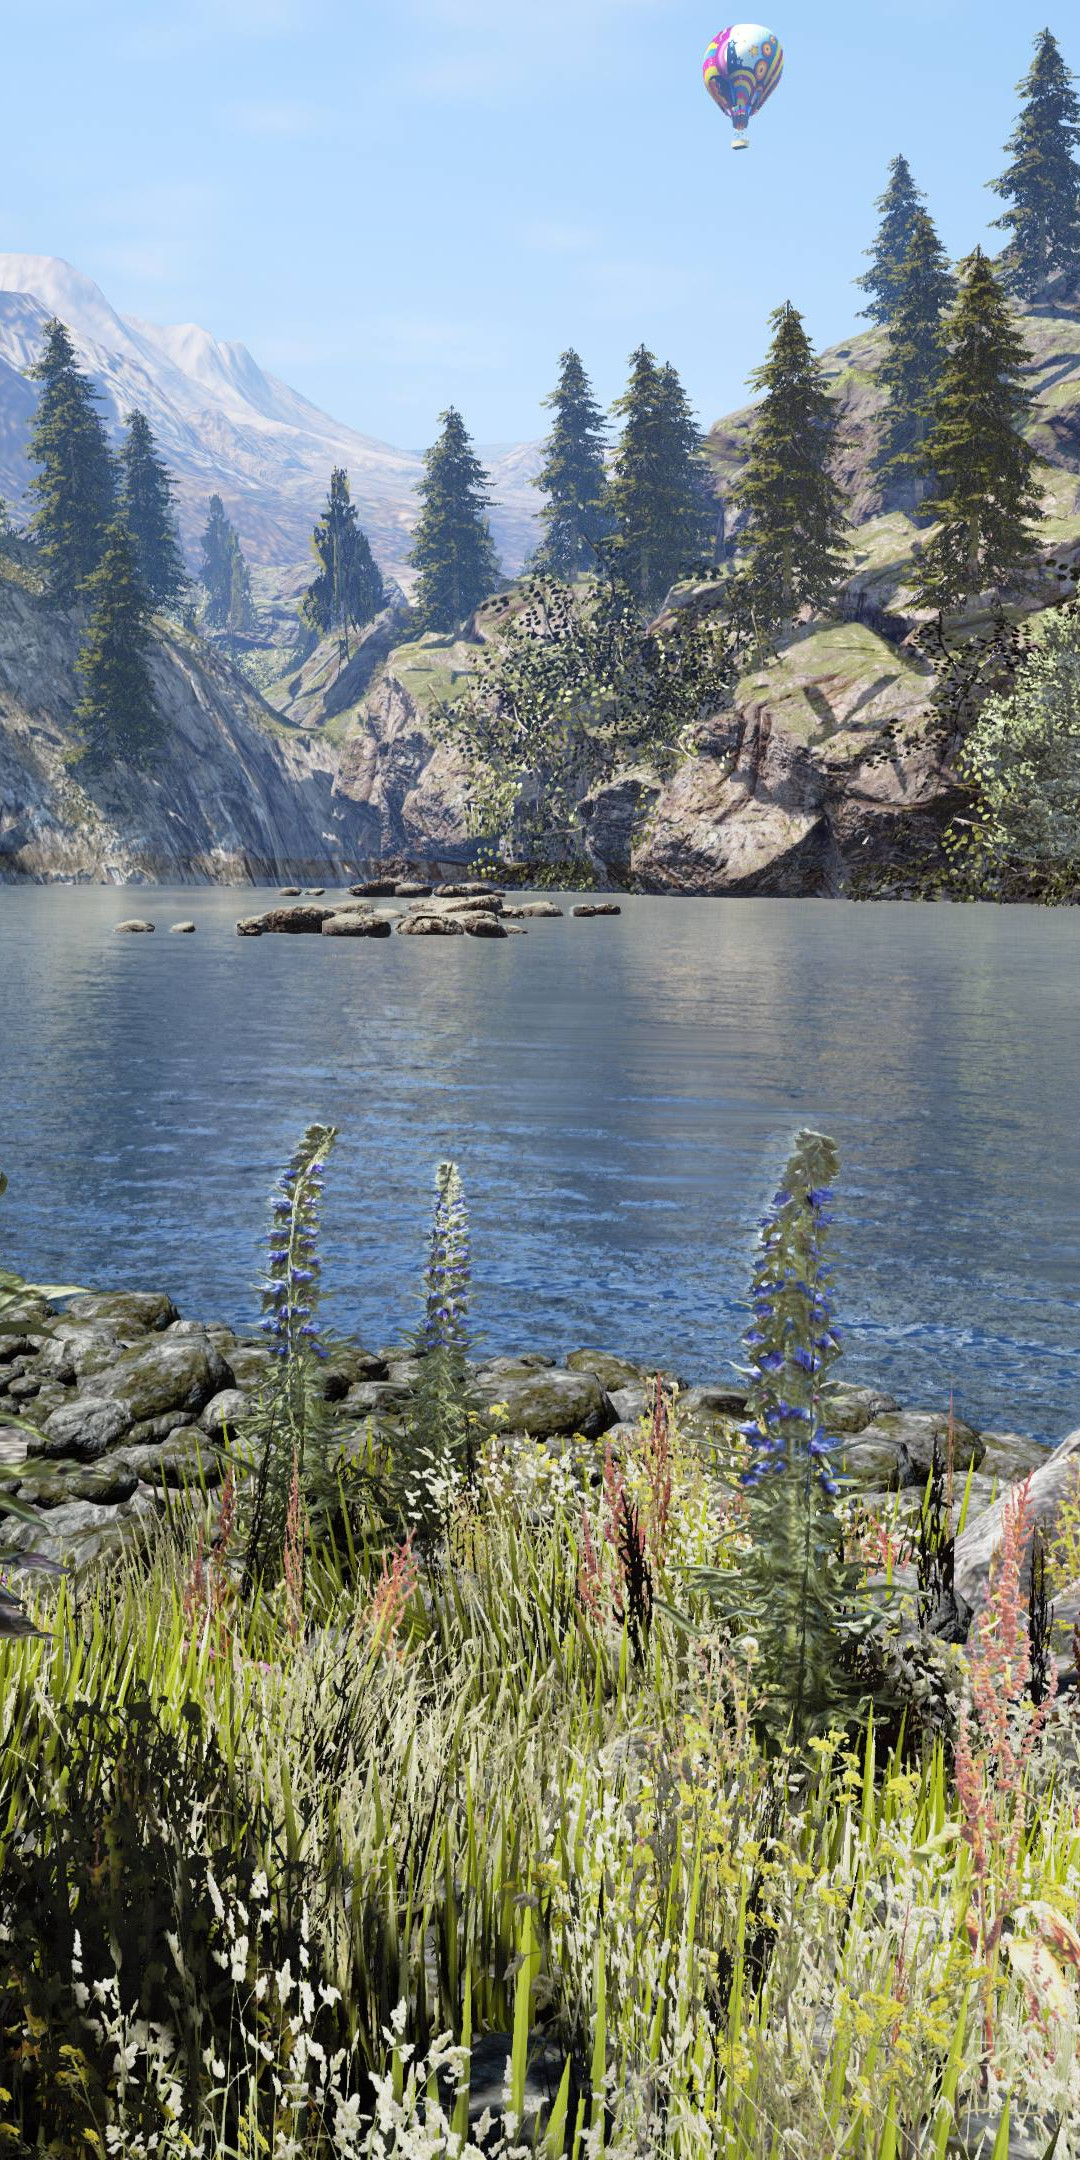
\includegraphics[width=\textwidth]{graphics/game_graphics}
    }
\end{frame}

\begin{frame}{UIs}
   \splitslide{0.7}{.7em}{
        \small

        While they look different, UIs generally use OpenGL or Direct3D as
        well. Everything is still made of textured \& shaded triangles. Anti-%
        aliasing, text fidelity, etc. are all more important while lighting
        effects are generally absent. Responsiveness is key, but the frame can
        be updated as needed, not every 30th of a second.

    }{
        
\includegraphics[width=\textwidth]{graphics/firefox_start}
    }
\end{frame}

\begin{frame}{Offline}
    \splitslide{0.7}{.7em}{
        \small

        Offline graphics are used when the medium is non-interactive (movies,
        advertisements, etc). Because the available resources are limited only
        by budget and patience, offline graphics have unmatched fidelity. CPUs
        are often used instead of GPUs because this allows for more advanced
        calculations. However, this comes at a cost. Individual frames may
        take days to render.

    }{
        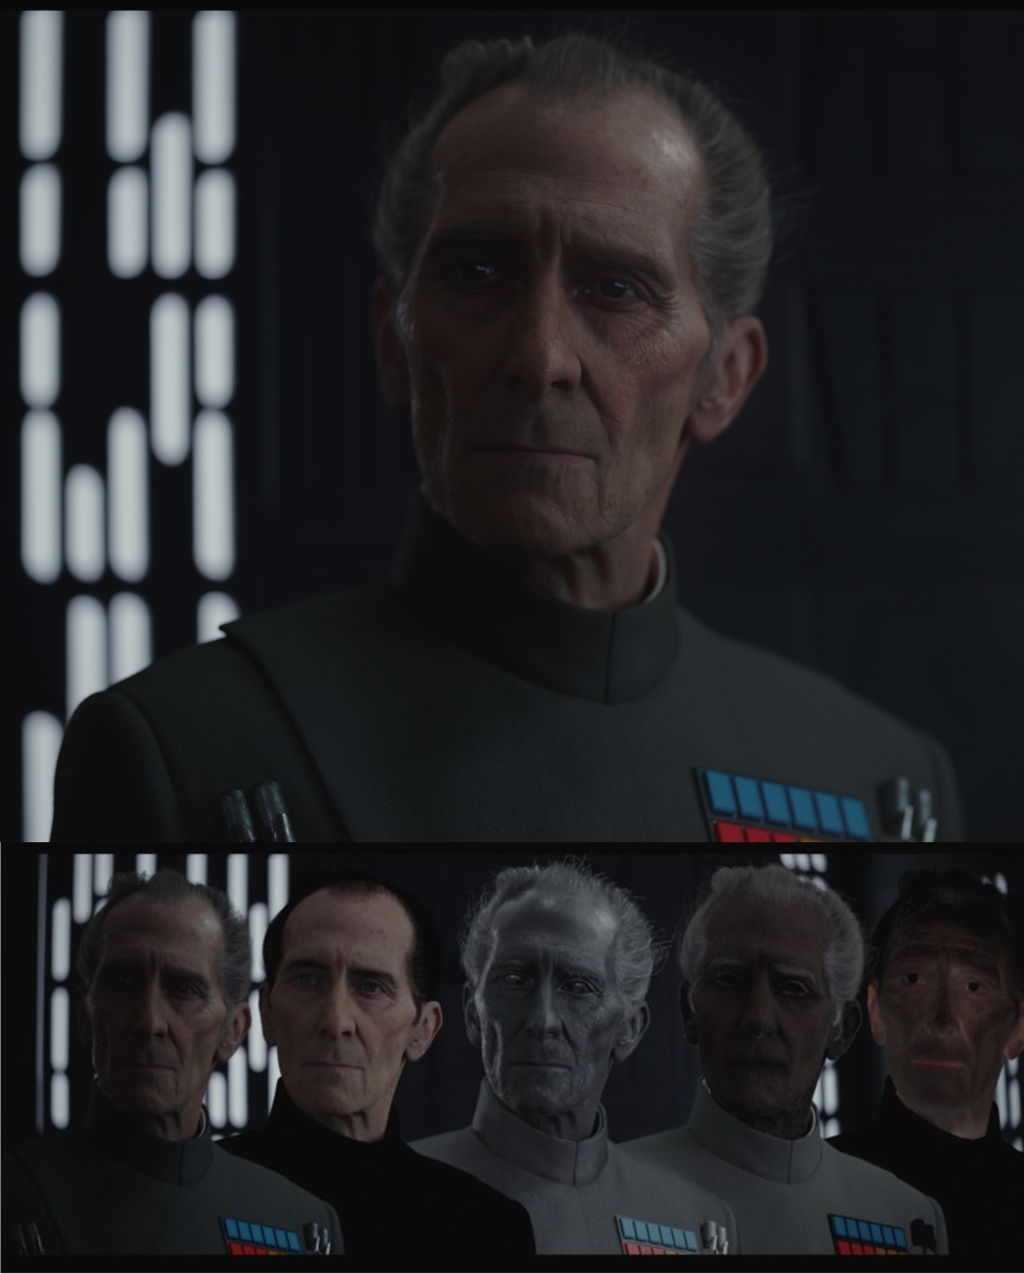
\includegraphics[width=\textwidth]{graphics/tarkin_combo} \\
        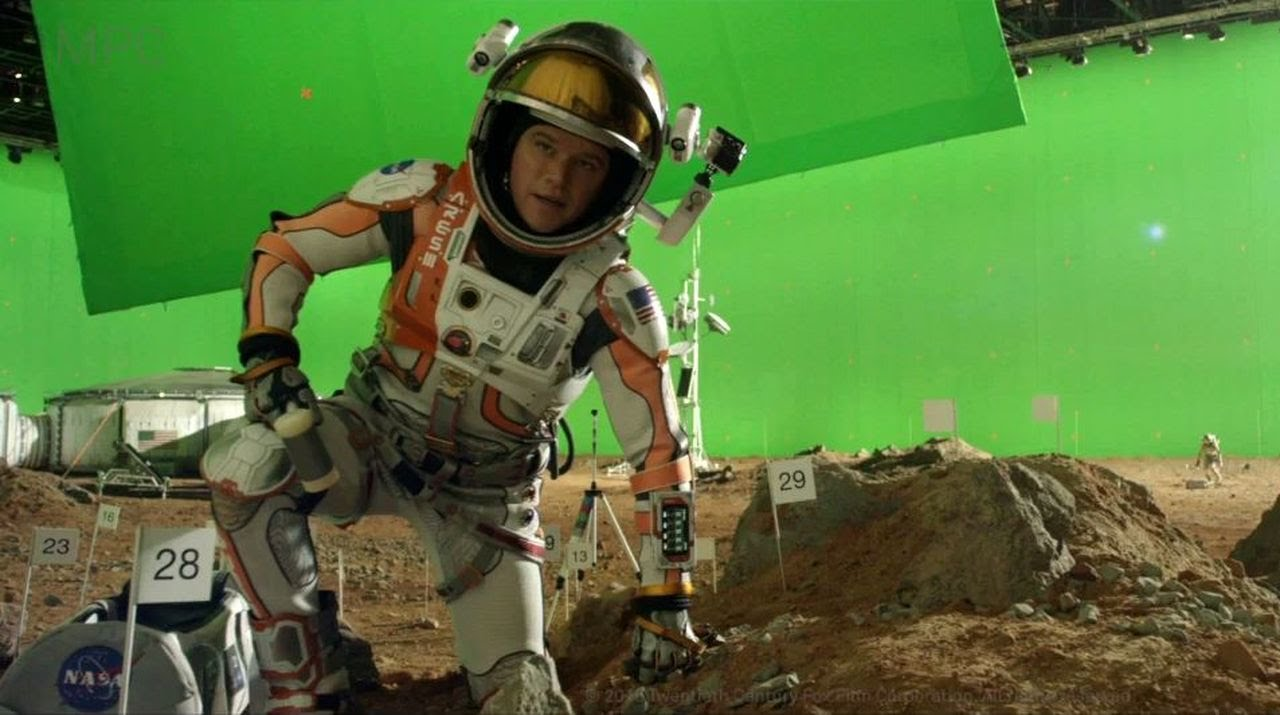
\includegraphics[width=\textwidth]{graphics/green_mars}
    }
\end{frame}

\section{History}

\begin{frame}{1950s \& 1960s}
    \splitslide{0.65}{.7em}{
        \small
        \begin{itemize}
            \item Military used computer controlled oscilloscopes to display strategic information
            \item Very simple graphical CAD programs and visualizers created
            \item Very first computer games
            \item Research into elementary 3D wireframe graphics
            \item Very early raster displays
        \end{itemize}
    }{
        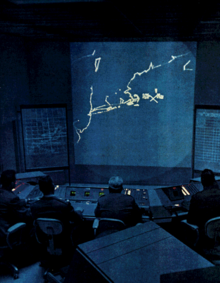
\includegraphics[width=\textwidth]{graphics/sage_control} \\
        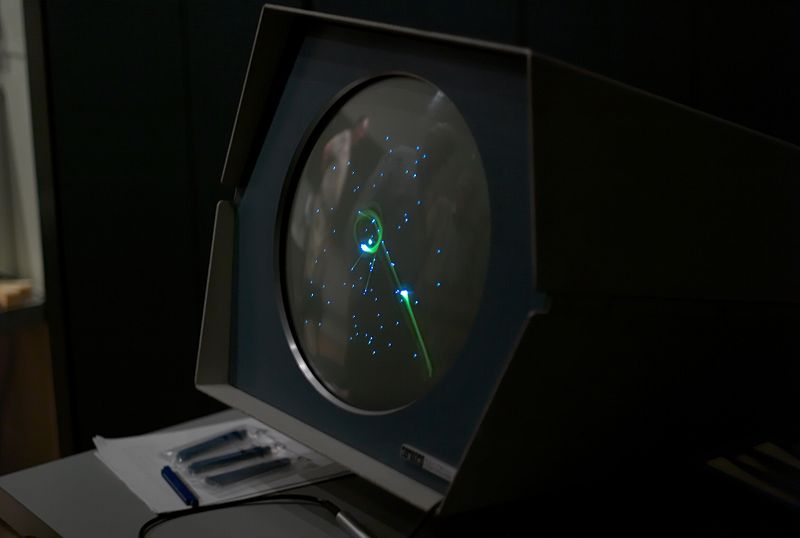
\includegraphics[width=\textwidth]{graphics/spacewar}
    }
\end{frame}

\begin{frame}{1970s \& 1980s}
    \splitslide{0.65}{.7em}{
        \small
        \begin{itemize}
            \item Basic lighting models such as Phong developed
            \item Low-res, 2D games become commercially available
            \item CGI starts to be used in Movies such as 1982's \textit{Wrath of Khan} and 1985's \textit{Young Sherlock Holmes}
            \item Modern GUIs are developed
            \item High-quality digital typesetting becomes commonplace
        \end{itemize}
    }{
        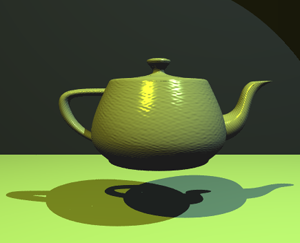
\includegraphics[width=\textwidth]{graphics/teapot_70s} \\
        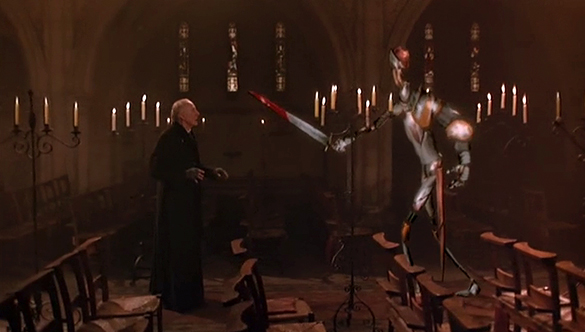
\includegraphics[width=\textwidth]{graphics/ysh_knight} \\
        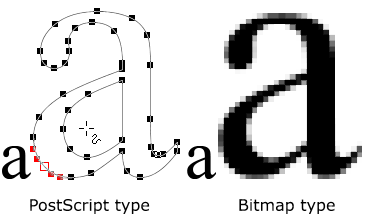
\includegraphics[width=\textwidth]{graphics/postscript_text}
    }
\end{frame}

\begin{frame}{1990s \& 2000s}
    \splitslide{0.65}{.7em}{
        \small
        \begin{itemize}
            \item Fidelity and performance are immensely increased
            \item Personal computers, 3D video games, and GUIs become ubiquitous
            \item OpenGL and Direct3D standardize hardware graphics support
            \item CGI becomes commonplace in Movies, advertisements, and TV 
            \item Global illumination and physically based rendering (PBR) techniques developed
        \end{itemize}
    }{
        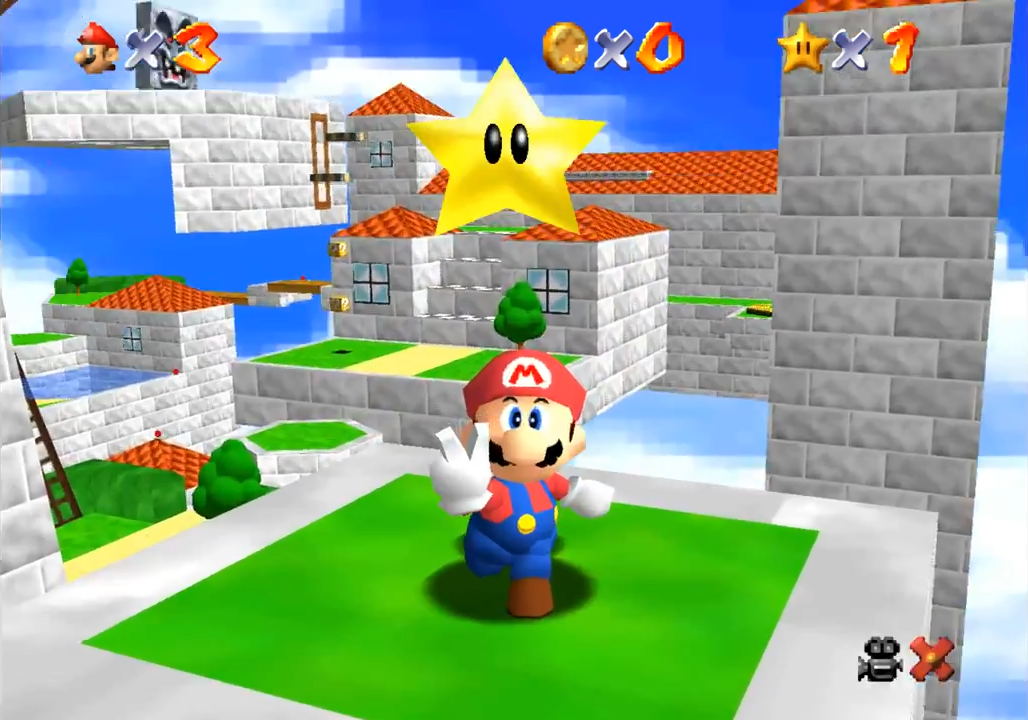
\includegraphics[width=\textwidth]{graphics/supermario64} \\
        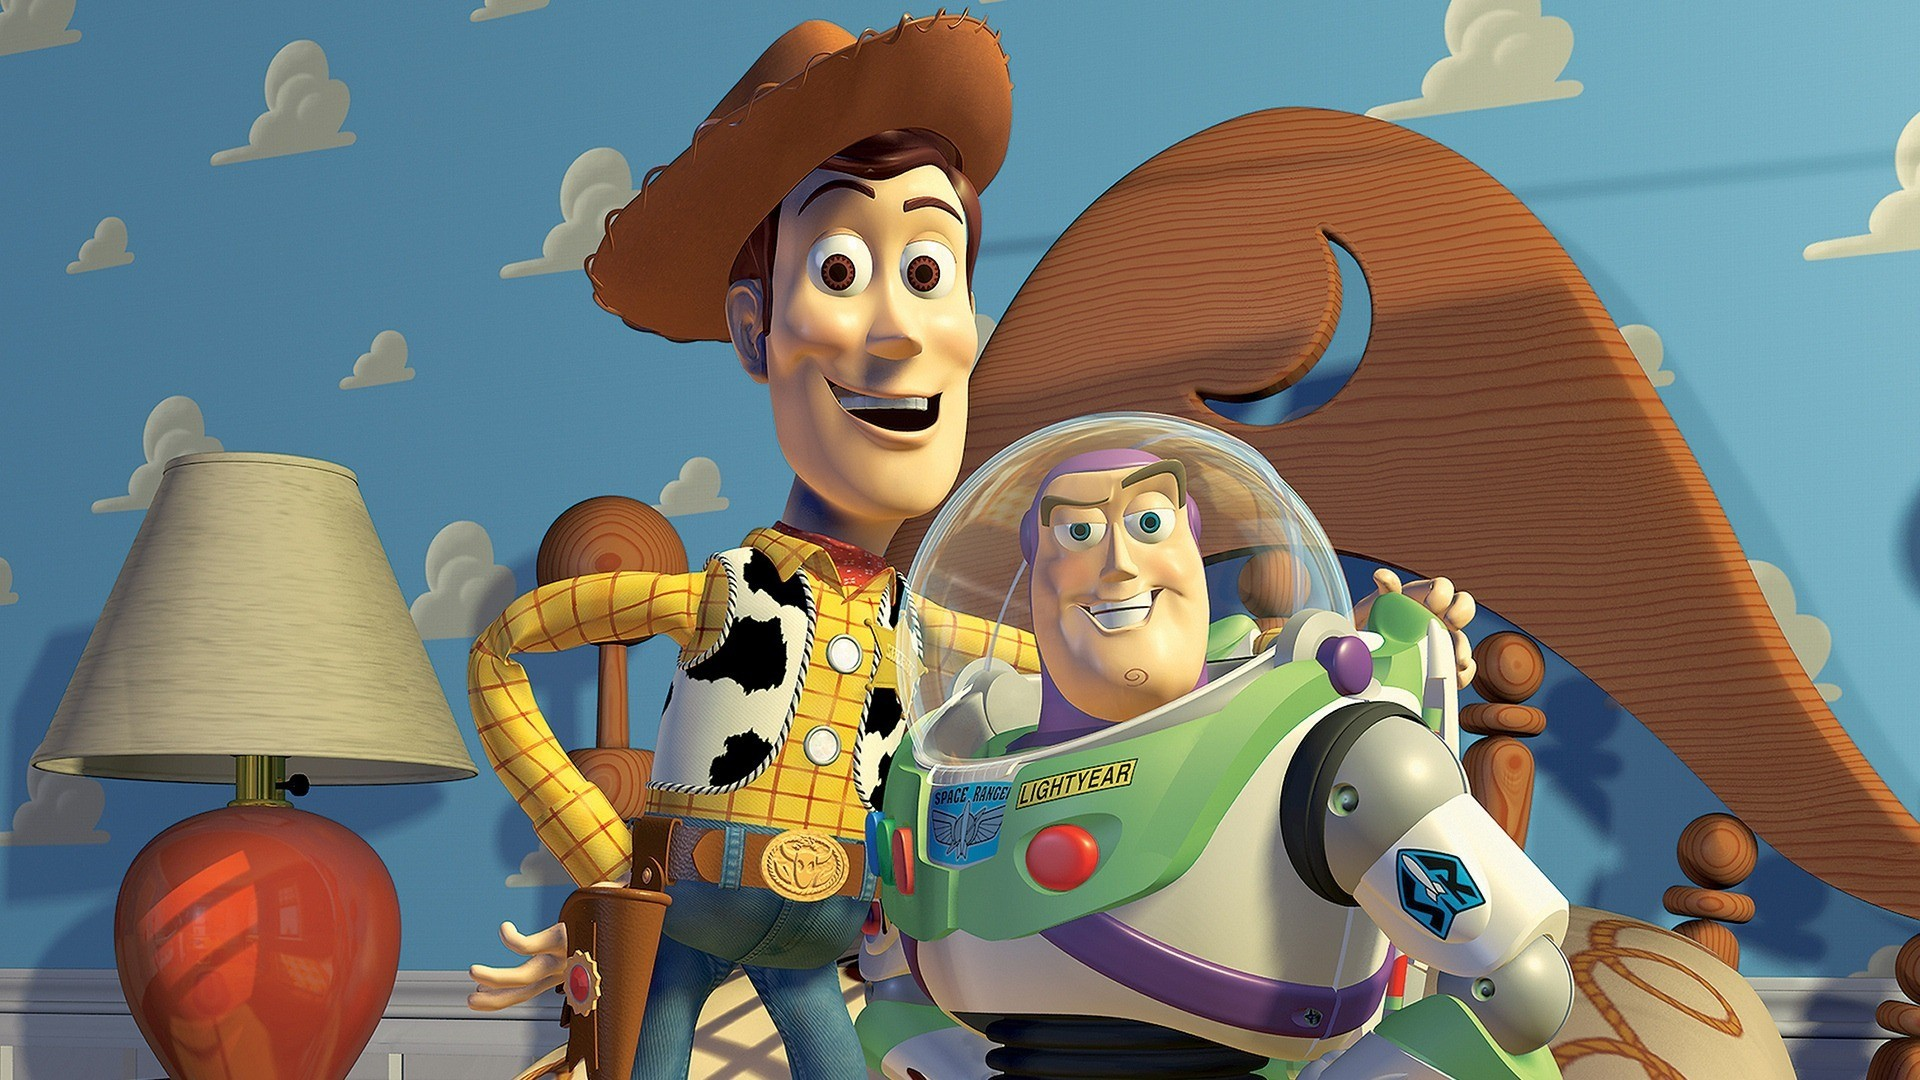
\includegraphics[width=\textwidth]{graphics/toy_story} \\
        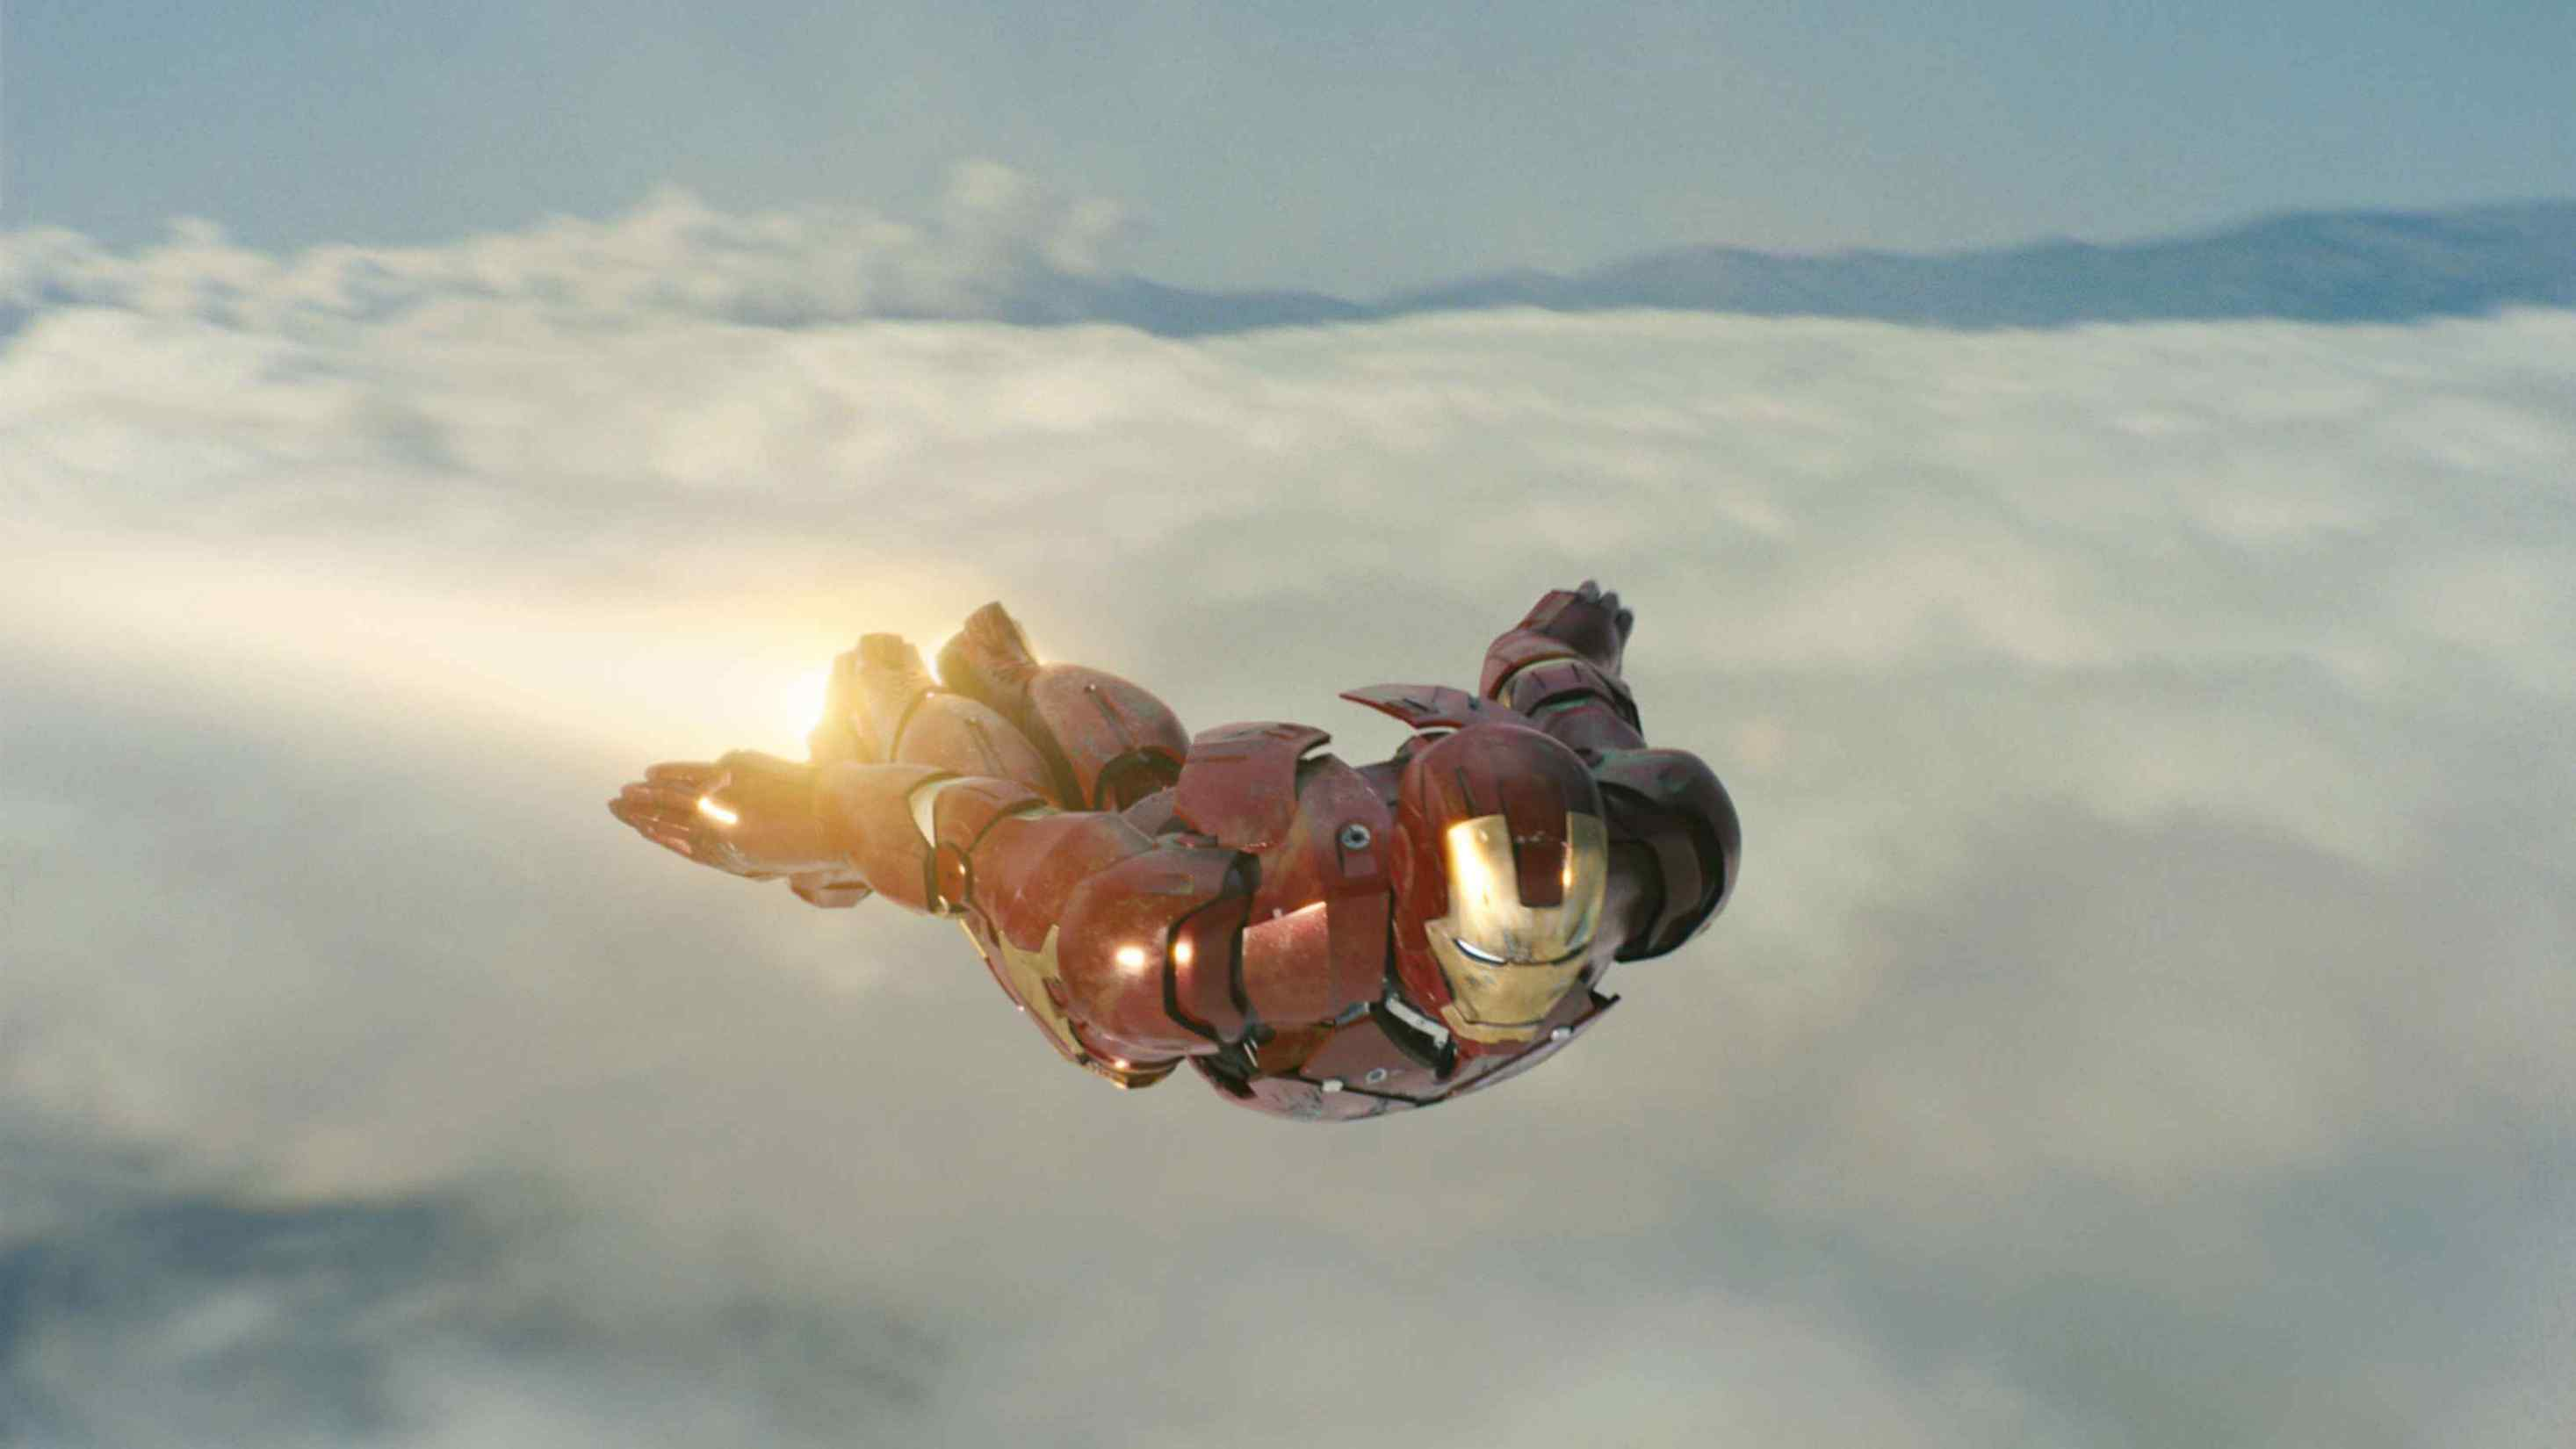
\includegraphics[width=\textwidth]{graphics/iron_man_2008}
    }
\end{frame}

\begin{frame}{Today}
    \splitslide{0.65}{.7em}{
        \small
        \begin{itemize}
            \item Given enough time, budget and expertise, offline graphics are photorealistic
            \item Particle and fluid simulations are extremely fast and accurate
            \item Realtime graphics make extensive use of shaders and PBR techniques
            \item UIs and offline graphics are increasingly GPU accelerated
            \item Linux and Mac have improved support for games and graphical software
        \end{itemize}
    }{
        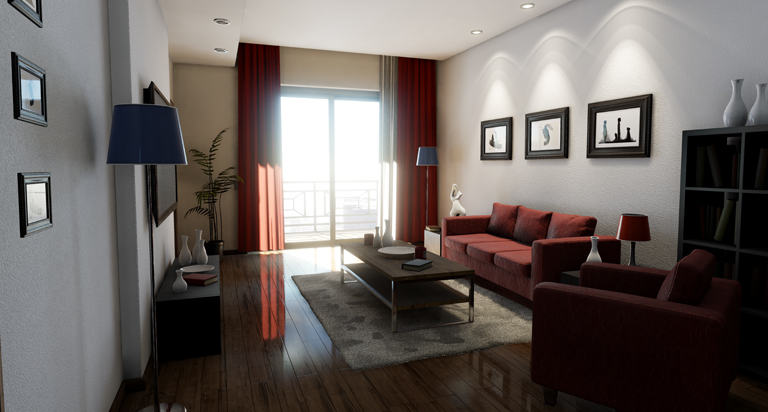
\includegraphics[width=\textwidth]{graphics/unreal4_damn.jpg} \\
        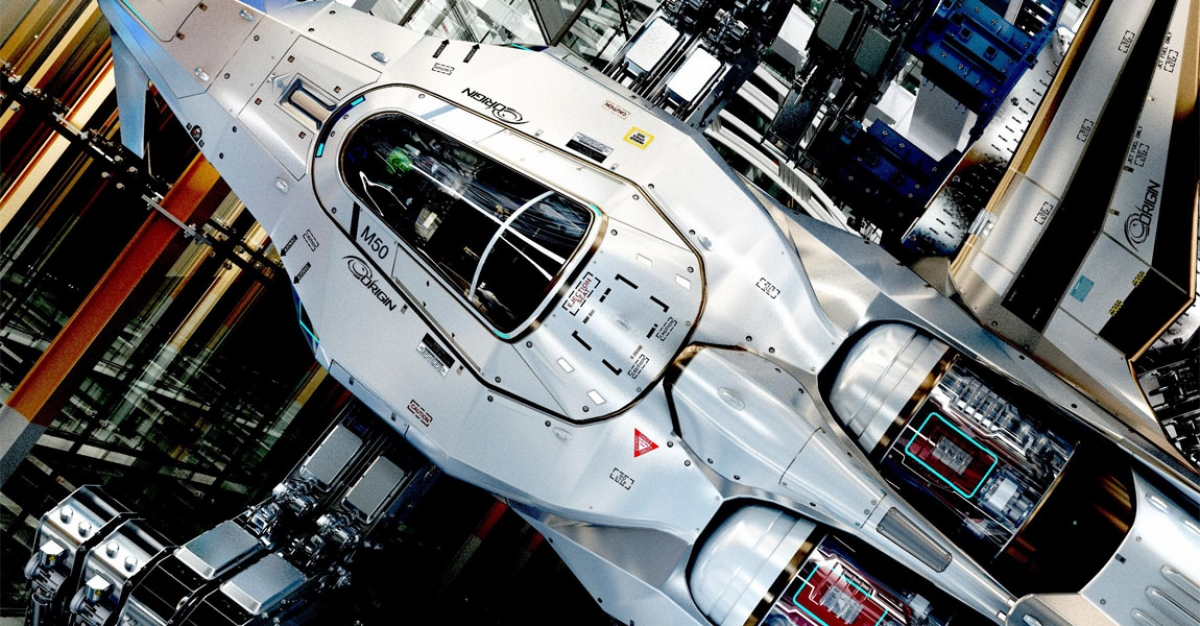
\includegraphics[width=\textwidth]{graphics/star_citizen_pbr} \\
        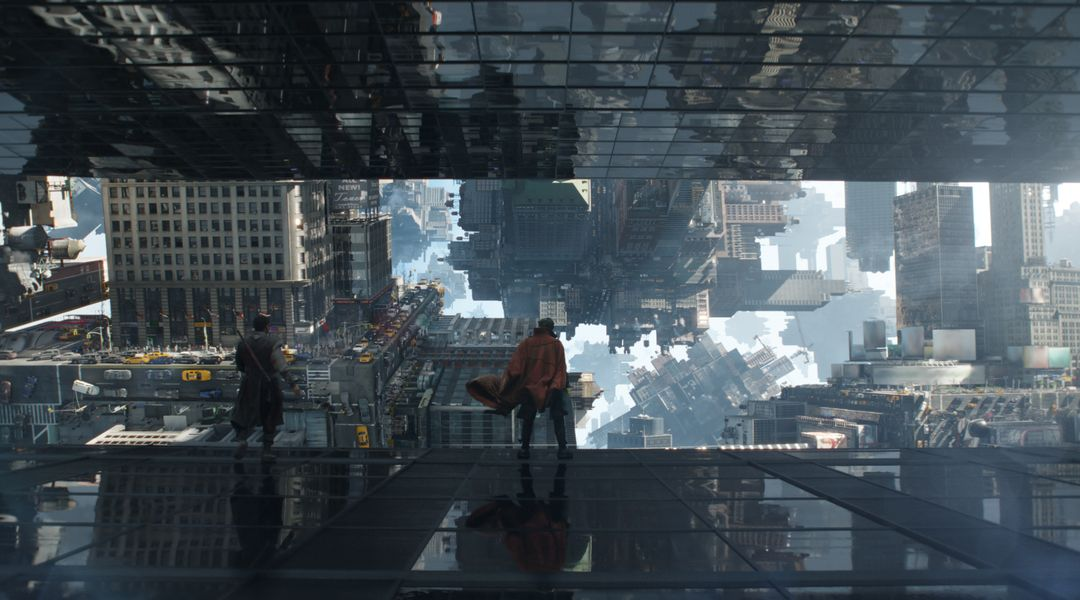
\includegraphics[width=\textwidth]{graphics/dr_strange} \\
        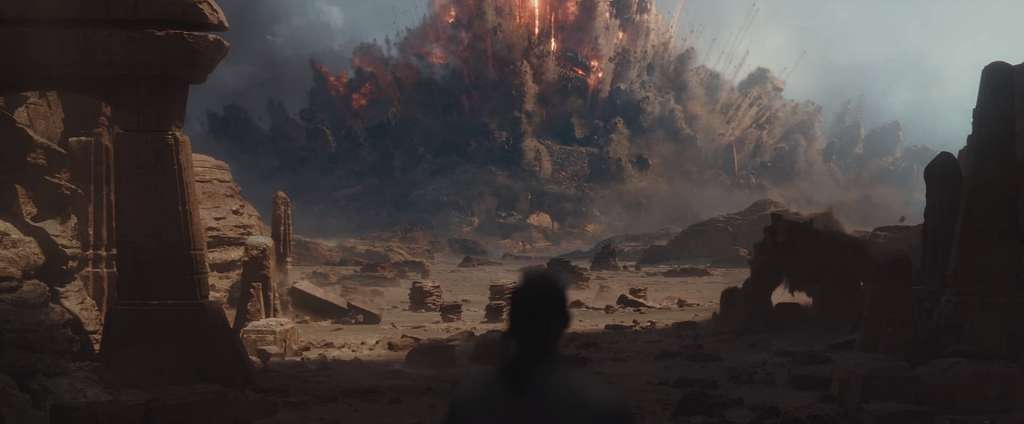
\includegraphics[width=\textwidth]{graphics/rogue_one_boom}
    }
\end{frame}

\section{Easy on the Eyes}

\begin{frame}{Text}
    \splitslide{0.65}{.7em}{
        \small

        The most common thing shown on screens is probably text. It is no
        wonder then that displaying text is one of the most sphisticated areas
        of computer graphics.

    }{
        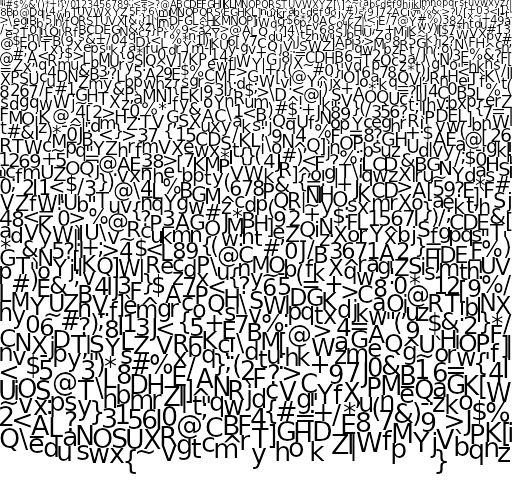
\includegraphics[width=\textwidth]{graphics/freetype_atlas} \\
        
\includegraphics[width=\textwidth]{graphics/subpixel_e}
    }
\end{frame}

\begin{frame}{Which is better?}
    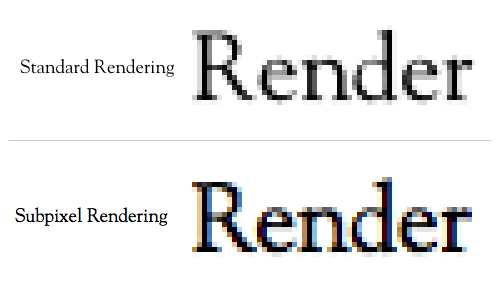
\includegraphics[width=\textwidth]{graphics/subpixel_side_by_side}
\end{frame}

\begin{frame}{Anti-aliasing}
    \splitslide{0.65}{.7em}{
        \small

        When small shapes (such as letters) are rasterized, details can find
        themselves squished into single pixels. In these cases, the color of
        the pixel is chosen arbitrarily depending on how the rasterization is
        performed. This creates all sorts of strange effects and hard edges,
        called "aliases".

        \vspace{1ex}

        The quality of the image can be greatly improved in some cases by
        using "anti-aliasing" algorithms and techniques.

    }{
        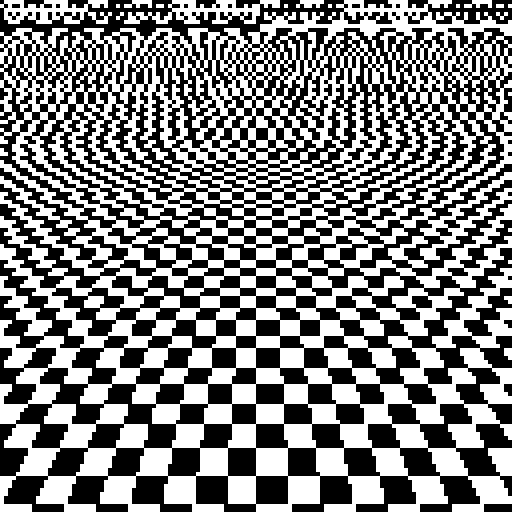
\includegraphics[width=\textwidth]{graphics/aliased} \\
        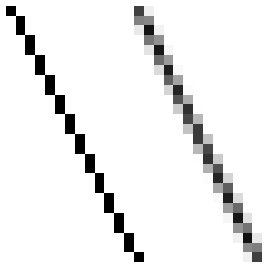
\includegraphics[width=\textwidth]{graphics/antialias_line}
    }
\end{frame}

\begin{frame}{Sub-pixels}
    \splitslide{0.65}{.7em}{
        \small

        Anti-aliasing can be taken further. After all, each pixel is really 3
        small red, green, and blue rectangles joined together. Clever people
        have figured out how to use these extra rectangles to further smooth
        the edges of letters and lines. This is why blown-up text (in an image
        editor) ends up being slightly colored on the edges.

    }{
        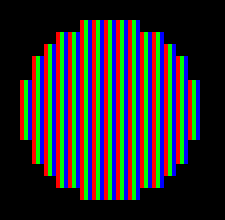
\includegraphics[width=\textwidth]{graphics/pixel_circle} \\
        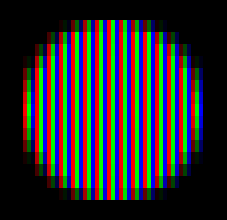
\includegraphics[width=\textwidth]{graphics/subpixel_circle}
    }
\end{frame}

\section{3D Shapes \& Geometry}

\begin{frame}{Meshes}
    \splitslide{0.65}{.7em}{
        \small

        3D shapes are often stored as a jumble of points (called verticies),
        scattered in space. These points are linked together into polygons,
        which form the surface of the model. Other methods of storing 3D
        shapes exist, such as the parametric forms used by Solid Works, but
        "meshes" are by far the most common. In fact, even when a different
        form is used, the model is almost always converted into a mesh for
        rendering anyway.

    }{
        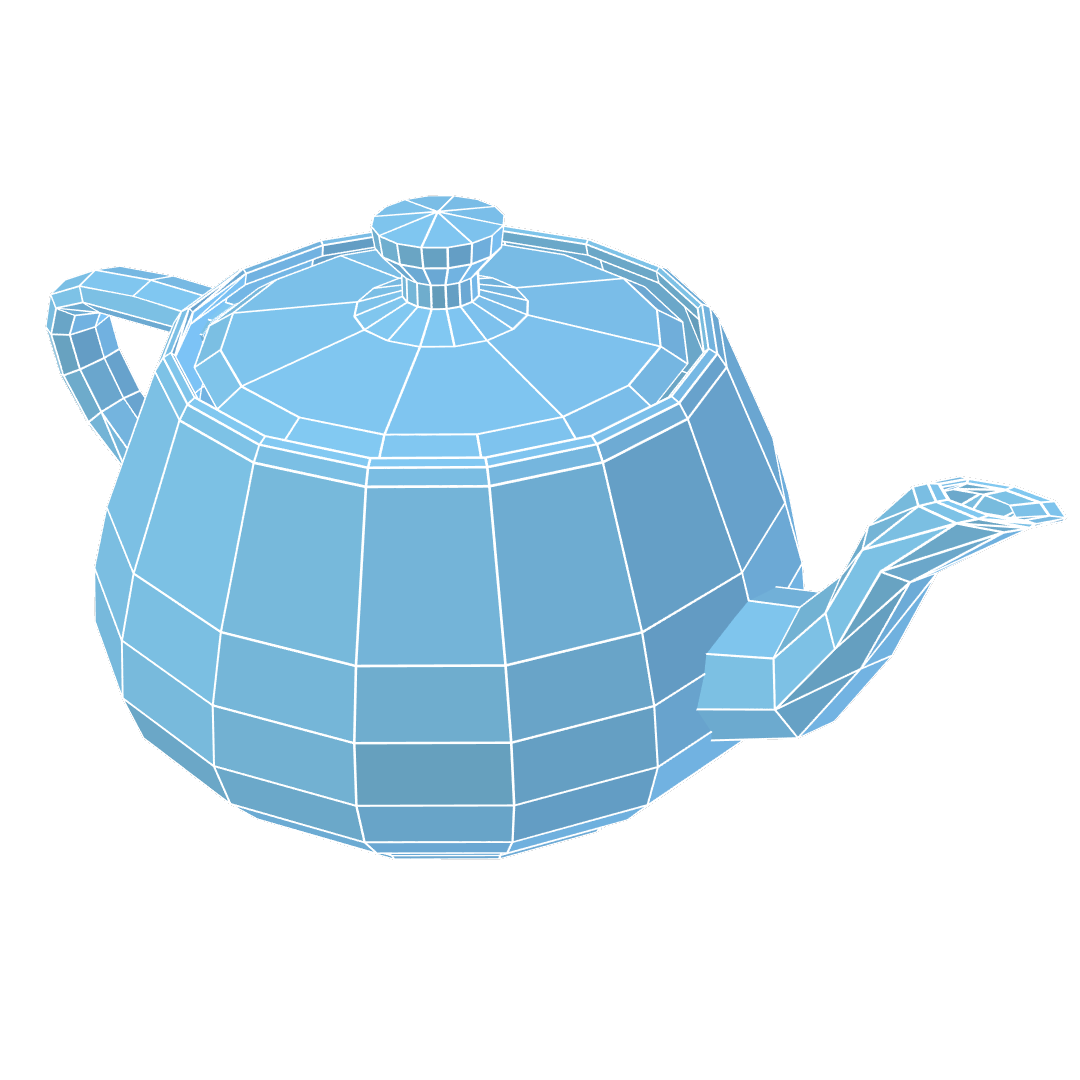
\includegraphics[width=\textwidth]{graphics/teapot_mesh}
    }
\end{frame}

\begin{frame}{Triangles}
    \splitslide{0.65}{.7em}{
        \small

        While any polygon could be used in a mesh, modern computer graphics
        deal almost exclusively in triangles. This is because triangles have
        some nice geometric properties that other shapes don't:

        \begin{itemize}
            \item It is very easy to test if a point is within a triangle (barycentric coordinates!)
            \item Any 3 points can be haphazardly connected together and still form a \underline{flat} triangle
            \item It is easy to calculate the direction a triangle is facing
        \end{itemize}
    }{
        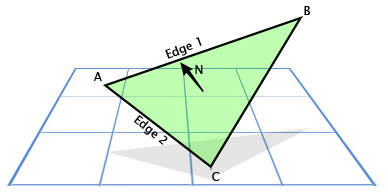
\includegraphics[width=\textwidth]{graphics/triangle}
    }
\end{frame}

\begin{frame}{Projection \& Rasterization}
    \splitslide{0.65}{.7em}{
        \small

        Meshes are 3D geometry. Screens are 2D pixels. Of the ways to convert
        between them, projection and rasterization is by far the simplest and
        most common. It works like so:

        \begin{enumerate}
            \item Rotate the scene such that $x$ is horizontal, $y$ is vertical, and $z$ is into the screen
            \item Do math for perspective
            \item Remove the $z$ value to "project" everything onto the $xy$ plane
            \item Iterate over the pixels the triangle covers
        \end{enumerate}
    }{
        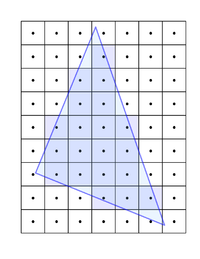
\includegraphics[width=\textwidth]{graphics/rasterization} \\
        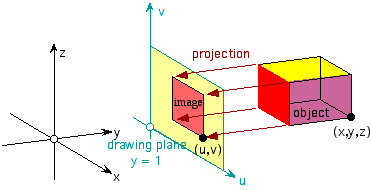
\includegraphics[width=\textwidth]{graphics/projection}
    }
\end{frame}

\begin{frame}{3D Modeling}
    \splitslide{0.5}{.2em}{
        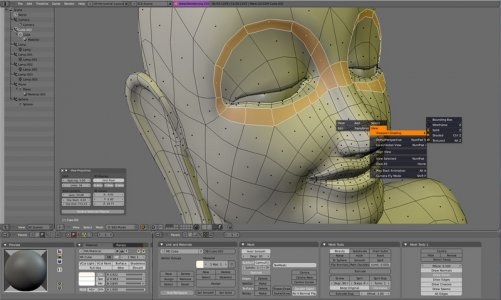
\includegraphics[width=\textwidth]{graphics/blender_eyes} \\
        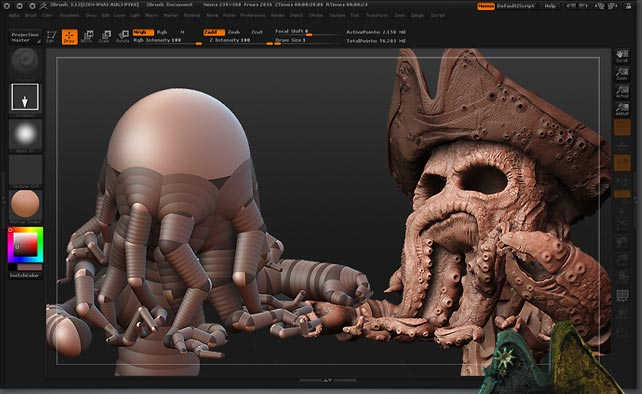
\includegraphics[width=\textwidth]{graphics/zbrush_squid}
    }{
        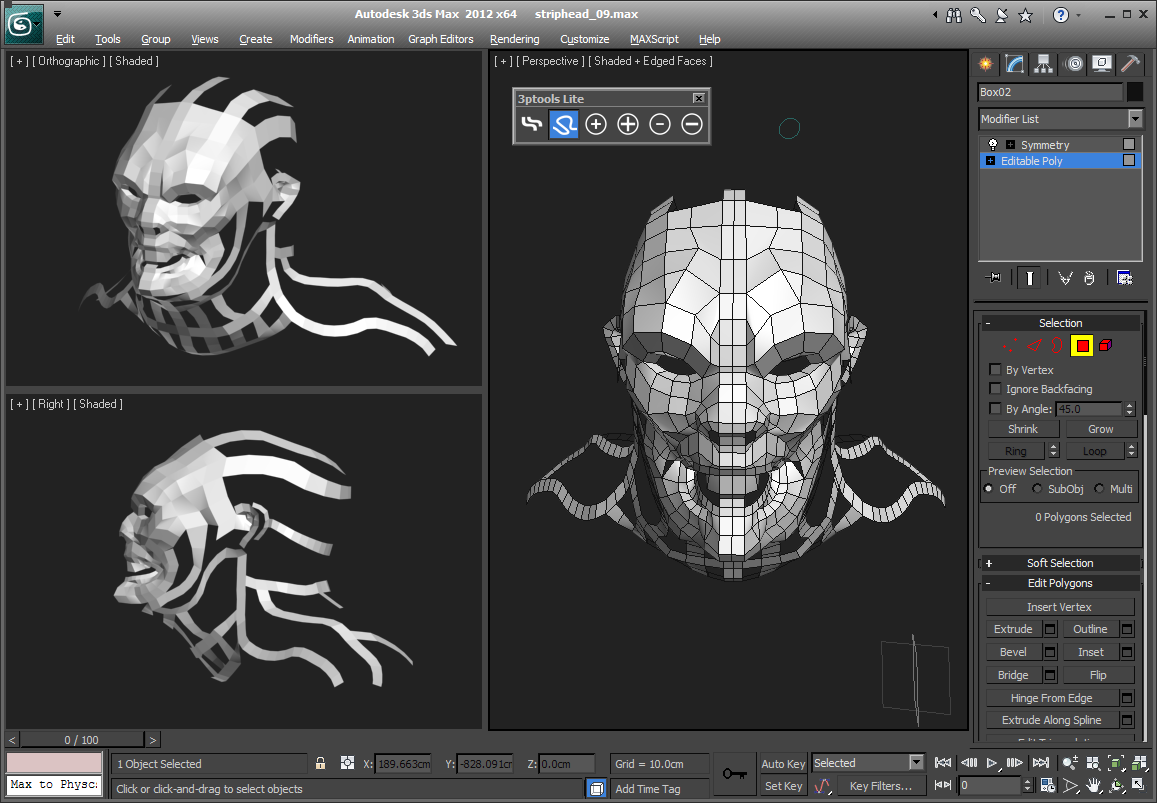
\includegraphics[width=\textwidth]{graphics/strip_head}
    }
        
\end{frame}

\section{Making it Pretty}

\begin{frame}{Textures}
    \splitslide{0.65}{.7em}{
        \small

         Textures are images (though they can contain more than colors) that
         are wrapped around 3D models. The exact method for this varies, but
         most of the time the wrapping is defined by a second set of
         coordinates attached to each vertex/point. This specifies where on
         the texture that point (and by extension, attached triangles) should
         lie.

         \vspace{1ex}

         This second set of positions is called the "UV map".

    }{
        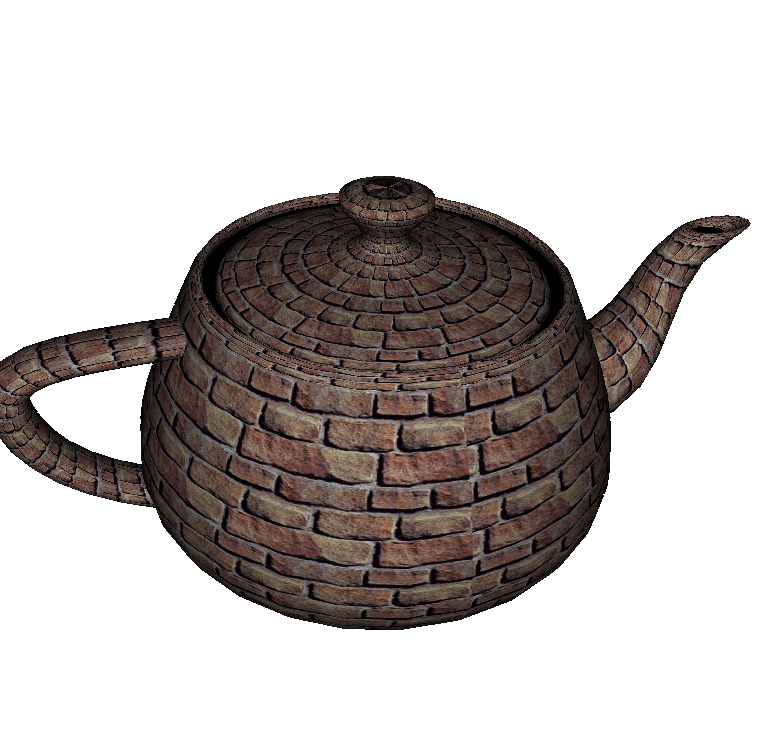
\includegraphics[width=\textwidth]{graphics/teapot_brick} \\
        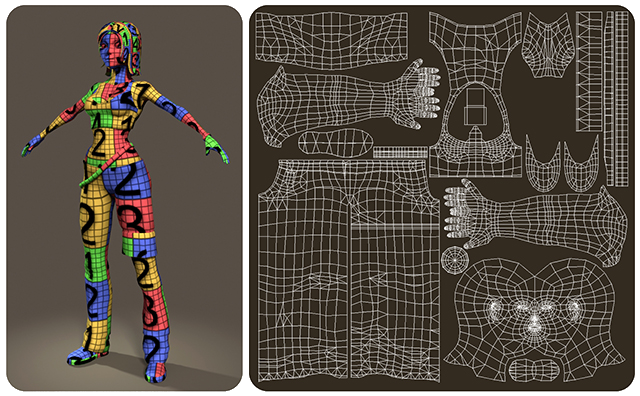
\includegraphics[width=\textwidth]{graphics/uv_map}
    }
\end{frame}

\begin{frame}{Mapping}
    \splitslide{0.65}{.7em}{
        \small

        Textures can be used to cover objects in all sorts of information. Not
        just color, but also material properties such as shininess and even
        precaculated lighting information.

        \vspace{1ex}

        More advanced techniques (such as bump, normal, and parallax mapping)
        can be used to fake bumps and other minute, shaded details on
        technically flat surfaces. Games use this extensively to make low-%
        resolution objects appear highly detailed (think screws, buckles,
        bricks, tree bark, ground texture, etc.)
 
    }{
        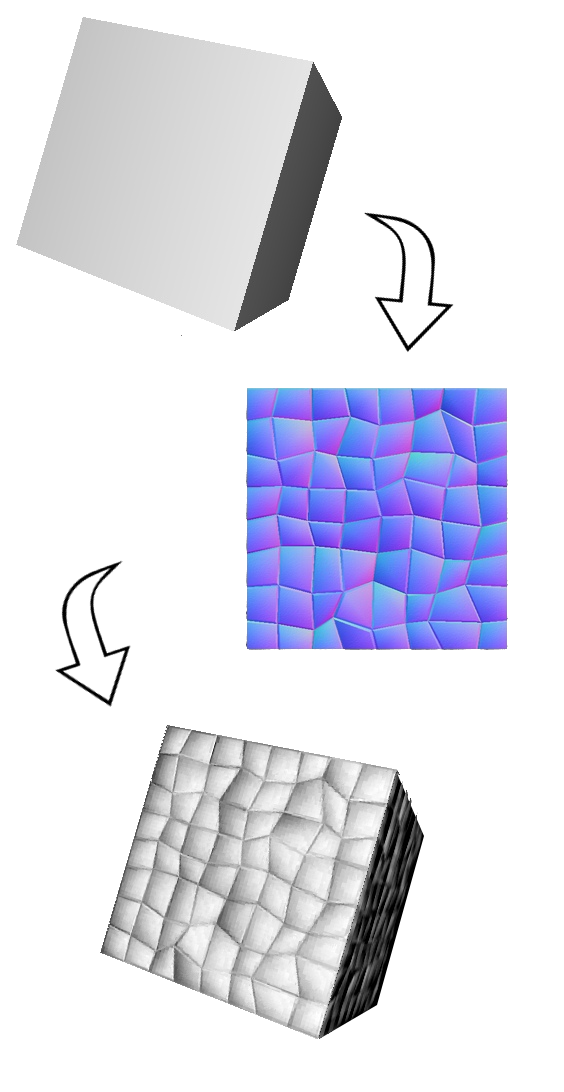
\includegraphics[width=\textwidth]{graphics/normal_map}
    }
\end{frame}

\begin{frame}{Phong}
    \splitslide{0.65}{.7em}{
        \small

        Phong is the simplest common shading model. It mixes diffuse shading
        (areas facing a light are brighter) and specular shading (areas that
        reflect light towards the camera are brighter) together. Think of how
        you would shade something with a pencil.

        \vspace{1ex}

        While this kind of works, it massively simplifies how real-world
        materials and lights interact. As a result, it looks downright fake.

    }{
        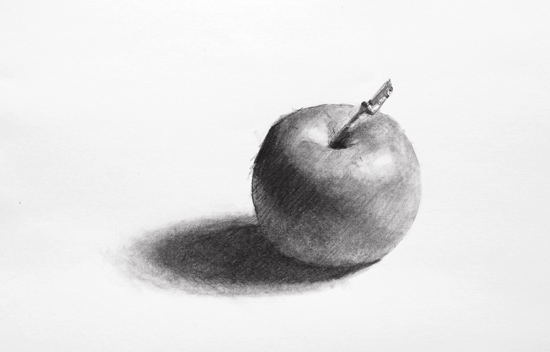
\includegraphics[width=\textwidth]{graphics/pencil_phong} \\
        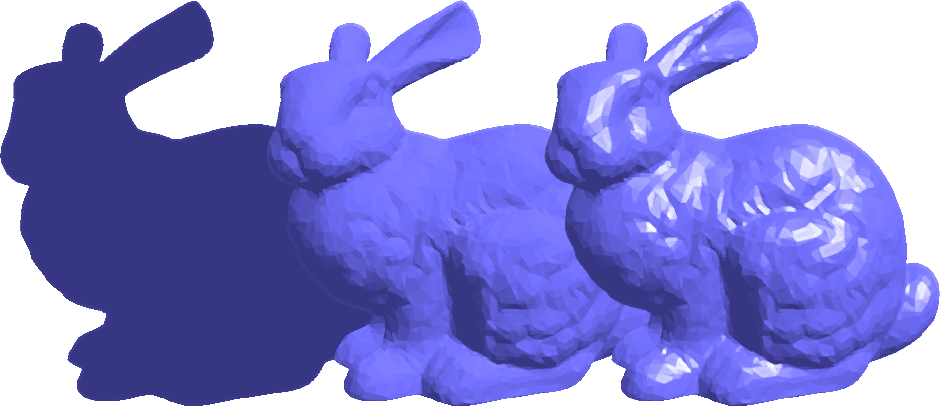
\includegraphics[width=\textwidth]{graphics/phong}
    }
\end{frame}

\begin{frame}{Painter's Algorithm}
    \splitslide{0.65}{.7em}{
        \small

        It goes without saying that things that are farther away should be
        hidden by things that are closer. The simplest way to do this in a
        computer is to draw the farther stuff first, so that when nearer stuff
        is drawn, it covers the previous stuff up.

        \vspace{1ex}

        However, this requires all the objects in the scene to be constantly
        resorted. It also can't deal with objects that mutually cover each
        other (like the Olympic rings).

        \vspace{1ex}

        That being said, there are still cases where the Painter's Algorithm
        is the only viable method.

    }{
        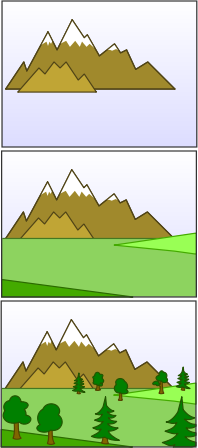
\includegraphics[width=\textwidth]{graphics/painters_alg}
    }
\end{frame}

\begin{frame}{Depth}
    \splitslide{0.65}{.7em}{
        \small

        A more common way to hide objects behind each other is to use a depth
        buffer. A depth buffer is a sort of distance image. In addition to
        keeping track of the color of each pixel, the distance from the camera
        to that pixel is also tracked. Then, whenever a new pixel is
        calculated, the computer checks whether is in front of or behind what
        is already there.

    }{
        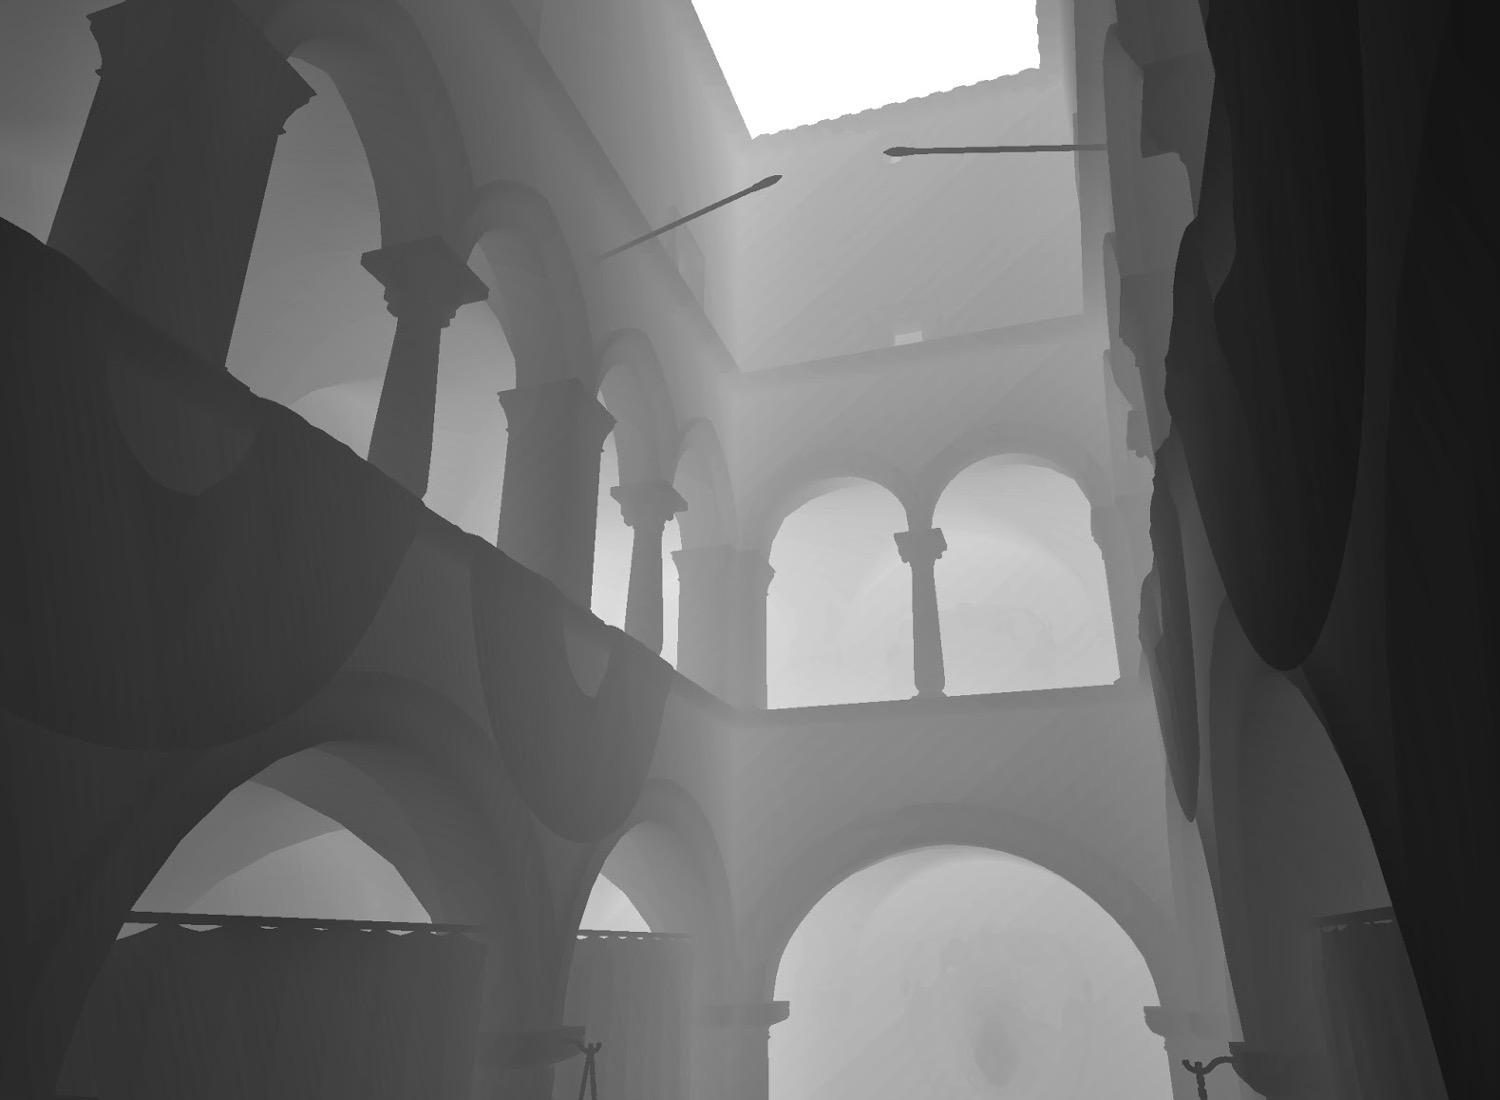
\includegraphics[width=\textwidth]{graphics/zbuffer2} \\
        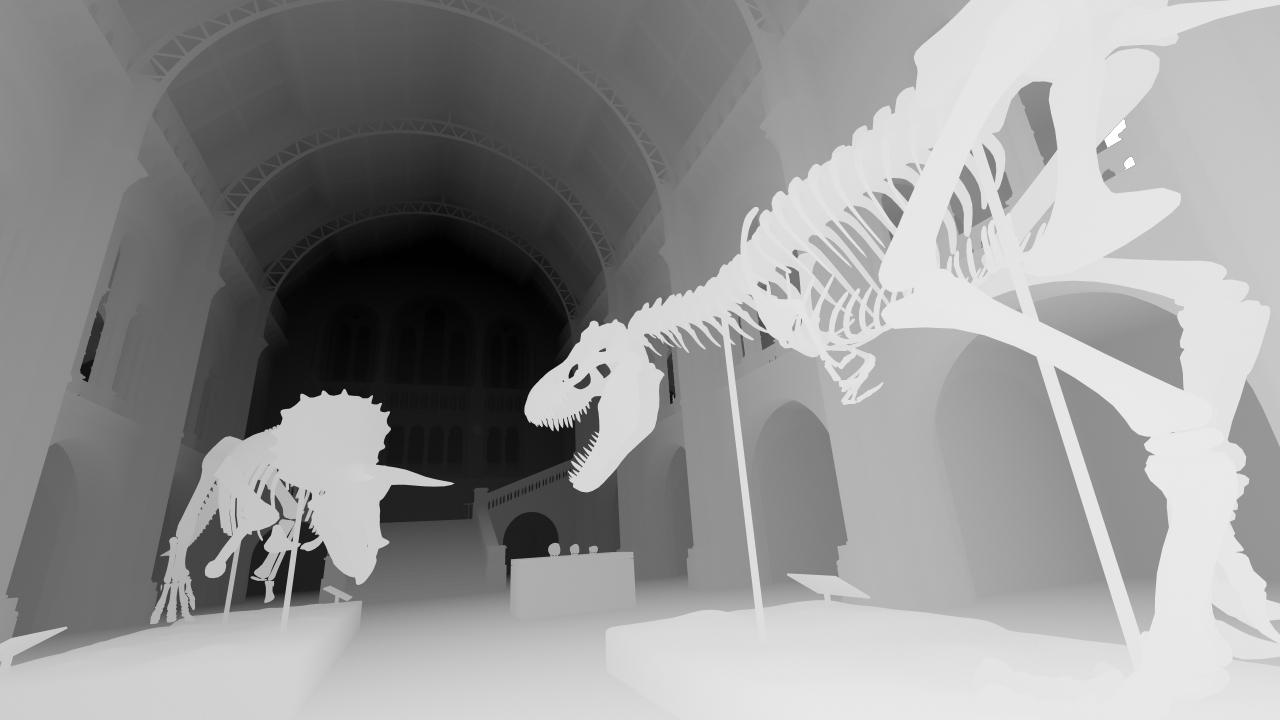
\includegraphics[width=\textwidth]{graphics/zbuffer}
    }
\end{frame}

\section{Effects}

\begin{frame}{Transparency}
    \splitslide{0.65}{.7em}{
        \small

        Simplicity, fidelity, speed. Pick one. Once transparency gets
        involved, the color of a given pixel is suddenly determined by more
        than one surface. This problem of mixing colors is common to pretty
        much all difficult-to-do things in computer graphics.

        \vspace{1ex}

        Most of the time transparency is handled by resorting back to the
        Painter's Algorithm. The rest of the scene can still use depth-%
        buffers, but it no longer makes sense to assign a single depth to
        those particular pixels.

    }{
        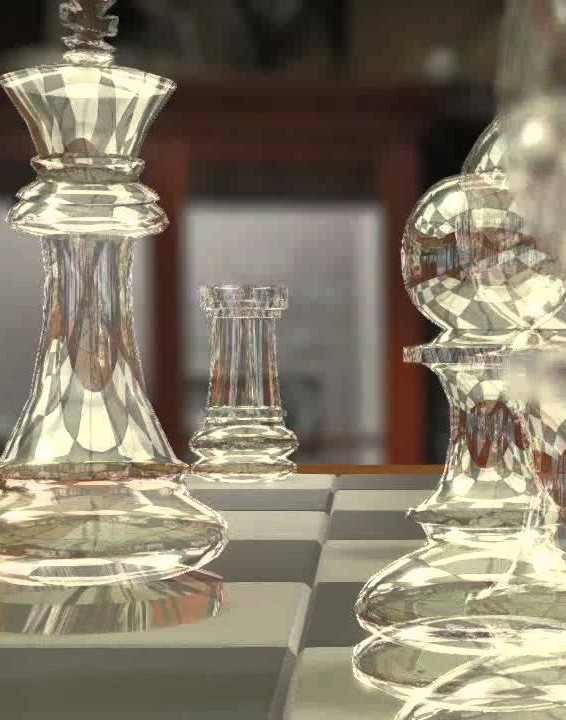
\includegraphics[width=\textwidth]{graphics/transparent}
    }
\end{frame}

\begin{frame}{Post-Processing}
    \splitslide{0.65}{.7em}{
        \small

        Texturing and shading is not always enough to make an image look good.
        Any photoshop guru can tell you how much a little tweaking can improve
        things. These "post-processing effects" arn't just used to make
        realtime graphics nicer, they are used to style-up photographs and
        videos as well.

    }{
        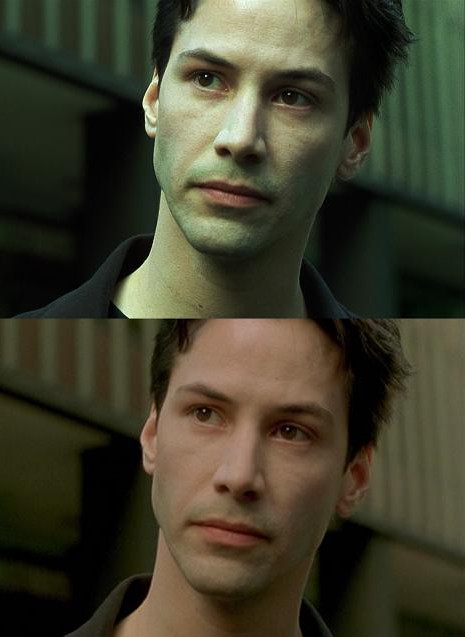
\includegraphics[width=\textwidth]{graphics/color_grading.jpeg}
    }
\end{frame}

\begin{frame}{Multipass Rendering}
    \splitslide{0.65}{.7em}{
        \small

        Post-processing can be taken even further. Instead of lighting and
        textured being performed as the shapes are rasterized, data from along
        the way can be saved in buffers and stapled together after the fact.

        \vspace{1ex}

        This has numerous benefits depending on how it is used. It is useful
        in realtime graphics because data from a single pass can be recycled
        to create multiple effects. Artists working on offline graphics like
        it because it lets them tweak shading and lighting without re-%
        rendering the whole scene.

    }{
        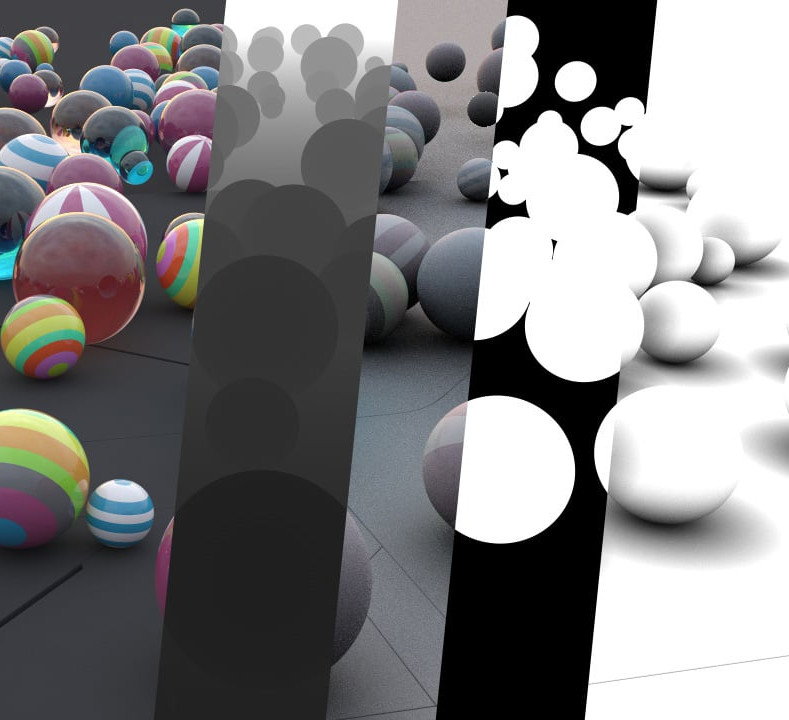
\includegraphics[width=\textwidth]{graphics/multipass}
    }
\end{frame}

\begin{frame}{Bluring}
    \splitslide{0.65}{.7em}{
        \small

        There are all sorts of algorithms to blur things, but the general case
        is pretty simple. The pixels around a point are weighted and averaged
        together.

        \vspace{1ex}

        Blurring is generally a post processing effect, but it can get more
        complicated when involving out-of-focus (field of view) effects.

    }{
        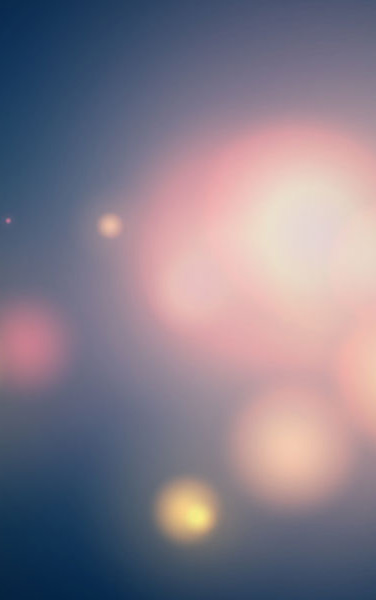
\includegraphics[width=\textwidth]{graphics/gaussian_blur}
    }
\end{frame}

\begin{frame}{Compositing}
    \splitslide{0.65}{.7em}{
        \small

        Compositing is mostly associated with movies and TV but it can apply
        to realtime visualizations and user interfaces as well. It is the
        process of combining graphics from multiple sources into a single
        image.

        \vspace{1ex}

        Green screening, color grading, atmospheric effects, etc. often fall
        under the umbrella of compositing.

    }{
        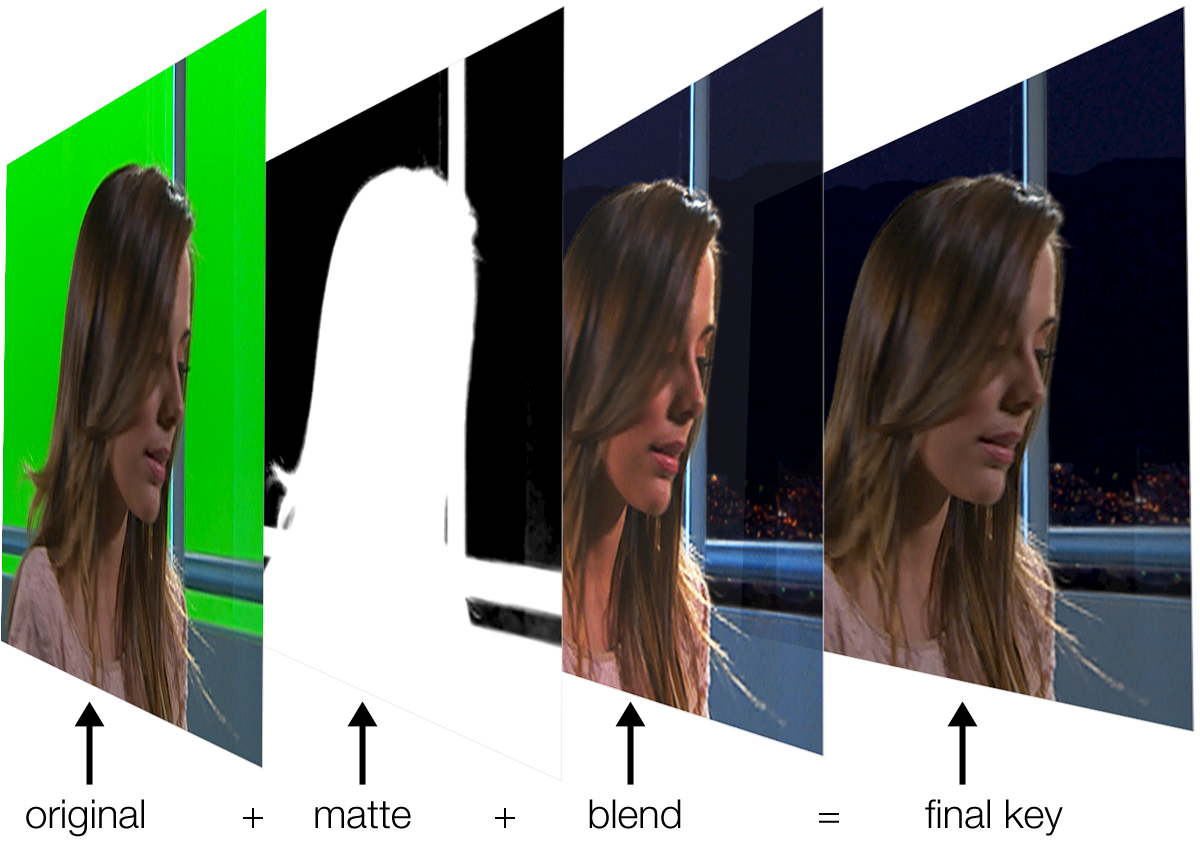
\includegraphics[width=\textwidth]{graphics/compositing_matte} \\
        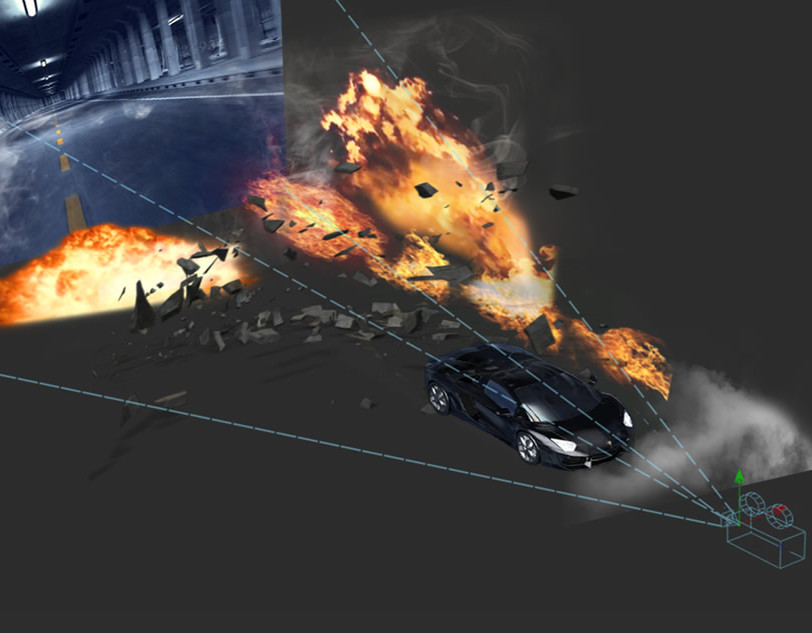
\includegraphics[width=\textwidth]{graphics/compositing}
    }
    \noindent
\end{frame}

\section{Realism}

\begin{frame}{Reflection}
    \splitslide{0.65}{.7em}{
        \small

        We have all seen images reflected in water, mirrors, shiny things,
        clean tables, computer screens, the list goes on. Achieving it in a
        computer is actually quite difficult. Often (especially for realtime
        applications) reflections are just cleverly distorted panoramas
        slapped onto the object of question. This breaks down on any
        complicated surface or scene however.

        \vspace{1ex}

        There is a REAL way of doing it, we will get to that in a few slides.

    }{
        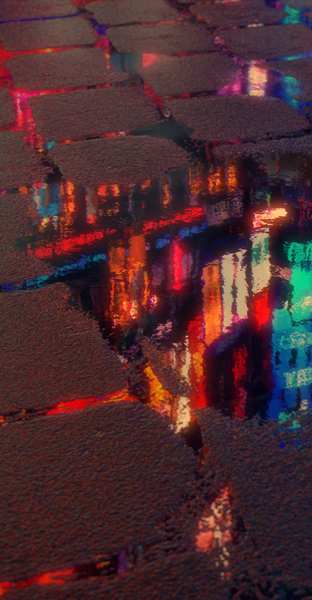
\includegraphics[width=\textwidth]{graphics/puddle-reflection}
    }
\end{frame}

\begin{frame}{Refraction}
    \splitslide{0.65}{.7em}{
        \small

        Refraction is even freakier and fakeir. You can \textit{kindof} do it
        in real time with fancy panoramas as well, but you don't want to know
        how. Just trust me.

    }{
        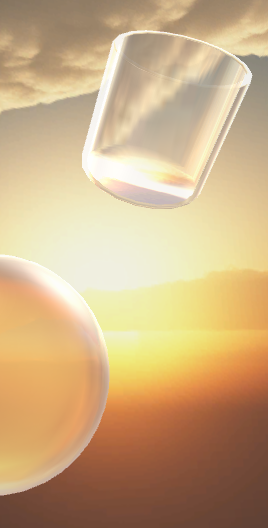
\includegraphics[width=\textwidth]{graphics/refraction}
    }
\end{frame}

\begin{frame}{Raytracing}
    \splitslide{0.65}{.7em}{
        \small

        So far we have been (mosty) talking about rasterization, just
        iterating through pixels. That is the only way to do things realtime,
        but if you remember physics 101 (or have even played with a flash
        light), you know that light doesn't work that way. It travels around
        in beams (or rays).

        \vspace{1ex}

        Raytracing is a technique where "rays" of light are followed backward,
        out of the camera and into the scene. They bounce off mirrors, refract
        through glass, and pick up color along the way.

    }{
        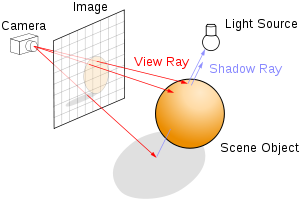
\includegraphics[width=\textwidth]{graphics/raytracing}
    }
\end{frame}

\begin{frame}{Fresnel \& PBR}
    \splitslide{0.65}{.7em}{
        \small

        Our Phong shading model is also hopelessly unrealistic. For a start,
        the reflectivity of an object actually changes depending on the angle
        you look at it from (a property called "fresnel"). How materials
        scatter light is really quite complicated in general. Taking that
        complexity into account is called Physically Based Rendering or PBR.

        \vspace{1ex}

        It is hot stuff these days.

    }{
        \includegraphics[width=\textwidth]{graphics/fresnel_spheres}
    }
\end{frame}

\begin{frame}{Global Illumination}
    \splitslide{0.65}{.7em}{
        \small

        We have also been assuming that the photons emitted from lights are
        somehow magical. Really everything is a light. A brightly illuminated
        red wall will reflect red light onto the rest of the scene. A corner
        is darker than the rest of the room because it is more shielded from
        rouge light bouncing around. A mirror isn't perfectly reflective, but
        actually blurs and scatters the image slightly. Shadows aren't on-or-%
        off, they blur towards the edges.

        \vspace{1ex}

        All of this is collectively called "global illumination" because light
        is a global property, it bounces and is emitted from everything, not
        just a few key sources.

    }{
        \includegraphics[width=\textwidth]{graphics/cornell_box}
    }
\end{frame}

\begin{frame}{Pathtracing}
    \splitslide{0.65}{.7em}{
        \small

        Which brings us to pathtracing. Pathtracing is the penultimate
        technique. Faster and more advanced methods exist in dissertations and
        prototypes, but pathtracing is the only thing in this presentation
        that can pass as photorealistic. It is more or less the method used
        today for CGI in movies, TV, advertisements, and art.

        \vspace{1ex}

        It is similar to raytracing, but instead of light bouncing directly,
        billions of theoretical and random paths are launched through the
        scene. Probibilities are calculated for each, and then after some some
        fancy statistics is applied, you get Iron Man.

    }{
        \includegraphics[width=\textwidth]{graphics/loungeroom}
    }
    \noindent
\end{frame}

\section{Wrapping it Up}

\end{document}